% Judul dokumen
\title{Buku Tugas Akhir ITS}
\author{Abel Marcel Renwarin}

% Pengaturan ukuran teks dan bentuk halaman dua sisi
\documentclass[12pt,twoside]{report}

% Pengaturan ukuran halaman dan margin
\usepackage[a4paper,top=30mm,left=30mm,right=20mm,bottom=25mm]{geometry}

% Pengaturan ukuran spasi
\usepackage[singlespacing]{setspace}

% Pengaturan detail pada file PDF
\usepackage[pdfauthor={\@author},bookmarksnumbered,pdfborder={0 0 0}]{hyperref}

% Pengaturan jenis karakter
\usepackage[utf8]{inputenc}

% Pengaturan pewarnaan
\usepackage[table,xcdraw]{xcolor}

% Pengaturan kutipan artikel
\usepackage[style=apa, backend=biber]{biblatex}

% Package lainnya
\usepackage{changepage}
\usepackage{enumitem}
\usepackage{eso-pic}
\usepackage{txfonts} % Font times
\usepackage{etoolbox}
\usepackage{graphicx}
\usepackage{lipsum}
\usepackage{longtable}
\usepackage{tabularx}
\usepackage{wrapfig}
\usepackage{float}


% Definisi untuk "Hati ini sengaja dikosongkan"
\patchcmd{\cleardoublepage}{\hbox{}}{
  \thispagestyle{empty}
  \vspace*{\fill}
  \begin{center}\textit{[Halaman ini sengaja dikosongkan]}\end{center}
  \vfill}{}{}

% Pengaturan penomoran halaman
\usepackage{fancyhdr}
\fancyhf{}
\renewcommand{\headrulewidth}{0pt}
\pagestyle{fancy}
\fancyfoot[LE,RO]{\thepage}
\patchcmd{\chapter}{plain}{fancy}{}{}
\patchcmd{\chapter}{empty}{plain}{}{}

% Command untuk bulan
\newcommand{\MONTH}{%
  \ifcase\the\month
  \or Januari% 1
  \or Februari% 2
  \or Maret% 3
  \or April% 4
  \or Mei% 5
  \or Juni% 6
  \or Juli% 7
  \or Agustus% 8
  \or September% 9
  \or Oktober% 10
  \or November% 11
  \or Desember% 12
  \fi}
\newcommand{\ENGMONTH}{%
  \ifcase\the\month
  \or January% 1
  \or February% 2
  \or March% 3
  \or April% 4
  \or May% 5
  \or June% 6
  \or July% 7
  \or August% 8
  \or September% 9
  \or October% 10
  \or November% 11
  \or December% 12
  \fi}

% Pengaturan format judul bab
\usepackage{titlesec}
\titleformat{\chapter}[display]{\bfseries\Large}{BAB \centering\Roman{chapter}}{0ex}{\vspace{0ex}\centering}
\titleformat{\section}{\bfseries\large}{\MakeUppercase{\thesection}}{1ex}{\vspace{1ex}}
\titleformat{\subsection}{\bfseries\large}{\MakeUppercase{\thesubsection}}{1ex}{}
\titleformat{\subsubsection}{\bfseries\large}{\MakeUppercase{\thesubsubsection}}{1ex}{}
\titlespacing{\chapter}{0ex}{0ex}{4ex}
\titlespacing{\section}{0ex}{1ex}{0ex}
\titlespacing{\subsection}{0ex}{0.5ex}{0ex}
\titlespacing{\subsubsection}{0ex}{0.5ex}{0ex}

% Atur variabel berikut sesuai namanya

% nama
\newcommand{\name}{Elon Reeve Musk}
\newcommand{\authorname}{Musk, Elon Reeve}
\newcommand{\nickname}{Elon}
\newcommand{\advisor}{Nikola Tesla, S.T., M.T}
\newcommand{\coadvisor}{Wernher von Braun, S.T., M.T}
\newcommand{\examinerone}{Dr. Galileo Galilei, S.T., M.Sc}
\newcommand{\examinertwo}{Friedrich Nietzsche, S.T., M.Sc}
\newcommand{\examinerthree}{Alan Turing, ST., MT}
\newcommand{\headofdepartment}{Prof. Albus Percival Wulfric Brian Dumbledore, S.T., M.T}

% identitas
\newcommand{\nrp}{0123 20 4000 0001}
\newcommand{\advisornip}{18560710 194301 1 001}
\newcommand{\coadvisornip}{18560710 194301 1 001}
\newcommand{\examineronenip}{18560710 194301 1 001}
\newcommand{\examinertwonip}{18560710 194301 1 001}
\newcommand{\examinerthreenip}{18560710 194301 1 001}
\newcommand{\headofdepartmentnip}{18810313 196901 1 001}

% judul
\newcommand{\tatitle}{KALKULASI ENERGI PADA ROKET LUAR ANGKASA BERBASIS \emph{ANTI-GRAVITASI}}
\newcommand{\engtatitle}{\emph{ANTI-GRAVITY BASED ENERGY CALCULATION ON OUTER SPACE ROCKETS}}

% tempat
\newcommand{\place}{Surabaya}

% jurusan
\newcommand{\studyprogram}{Teknik Dirgantara}
\newcommand{\engstudyprogram}{Aerospace Engineering}

% fakultas
\newcommand{\faculty}{Teknologi Dirgantara}
\newcommand{\engfaculty}{Aerospace Technology}

% singkatan fakultas
\newcommand{\facultyshort}{FTMD}
\newcommand{\engfacultyshort}{FMAE}

% departemen
\newcommand{\department}{Teknik Dirgantara}
\newcommand{\engdepartment}{Aerospace Engineering}

% kode mata kuliah
\newcommand{\coursecode}{TD123456}


% Tambahkan format tanda hubung yang benar di sini
\hyphenation{
  ro-ket
  me-ngem-bang-kan
  per-hi-tu-ngan
  tek-no-lo-gi
  me-la-ku-kan
  ber-so-si-al-i-sa-si
}

% Menambahkan resource daftar pustaka
\addbibresource{pustaka/pustaka.bib}

% Pengaturan format potongan kode
\usepackage{listings}
\definecolor{comment}{RGB}{0,128,0}
\definecolor{string}{RGB}{255,0,0}
\definecolor{keyword}{RGB}{0,0,255}
\lstdefinestyle{codestyle}{
  commentstyle=\color{comment},
  stringstyle=\color{string},
  keywordstyle=\color{keyword},
  basicstyle=\footnotesize\ttfamily,
  numbers=left,
  numberstyle=\tiny,
  numbersep=5pt,
  frame=lines,
  breaklines=true,
  prebreak=\raisebox{0ex}[0ex][0ex]{\ensuremath{\hookleftarrow}},
  showstringspaces=false,
  upquote=true,
  tabsize=2,
}
\lstset{style=codestyle}

% Isi keseluruhan dokumen
\begin{document}

% Sampul luar Bahasa Indonesia
\newcommand\covercontents{sampul/konten-id.tex}
\AddToShipoutPictureBG*{
  \AtPageLowerLeft{
    % Ubah nilai berikut jika posisi horizontal background tidak sesuai
    \hspace{-3.25mm}

    % Ubah nilai berikut jika posisi vertikal background tidak sesuai
    \raisebox{0mm}{
      
\includegraphics[width=\paperwidth,height=\paperheight]{sampul/gambar/sampul-luar.png}
    }
  }
}

% Menyembunyikan nomor halaman
\thispagestyle{empty}

% Pengaturan margin untuk menyesuaikan konten sampul
\newgeometry{
  top=55mm,
  left=30mm,
  right=20mm,
  bottom=20mm
}

\begin{flushleft}

  % Pemilihan font sans serif
  \sffamily

  % Pemilihan warna font putih
  \color{white}

  % Pemilihan font bold
  \fontseries{bx}
  \selectfont
  \begin{spacing}{1.5}
    \input{\covercontents}
  \end{spacing}

\end{flushleft}

\restoregeometry


% Atur ulang penomoran halaman
\setcounter{page}{1}

% Sampul dalam Bahasa Indonesia
\renewcommand\covercontents{sampul/konten-id.tex}
\AddToShipoutPictureBG*{
  \AtPageLowerLeft{
    % Ubah nilai berikut jika posisi horizontal background tidak sesuai
    \hspace{-4mm}

    % Ubah nilai berikut jika posisi vertikal background tidak sesuai
    \raisebox{0mm}{
      
\includegraphics[width=\paperwidth,height=\paperheight]{sampul/gambar/sampul-luar-tipis.png}
    }
  }
}

% Menyembunyikan nomor halaman
\thispagestyle{empty}

% Pengaturan margin untuk menyesuaikan konten sampul
\newgeometry{
  top=65mm,
  left=30mm,
  right=30mm,
  bottom=20mm
}

\begin{flushleft}

  % Pemilihan font sans serif
  \sffamily

  % Pemilihan font bold
  \fontseries{bx}
  \selectfont
  \begin{spacing}{1.5}
    \input{\covercontents}
  \end{spacing}

\end{flushleft}

\restoregeometry

\clearpage
\cleardoublepage

% Sampul dalam Bahasa Inggris
\renewcommand\covercontents{sampul/konten-en.tex}
\AddToShipoutPictureBG*{
  \AtPageLowerLeft{
    % Ubah nilai berikut jika posisi horizontal background tidak sesuai
    \hspace{-4mm}

    % Ubah nilai berikut jika posisi vertikal background tidak sesuai
    \raisebox{0mm}{
      
\includegraphics[width=\paperwidth,height=\paperheight]{sampul/gambar/sampul-luar-tipis.png}
    }
  }
}

% Menyembunyikan nomor halaman
\thispagestyle{empty}

% Pengaturan margin untuk menyesuaikan konten sampul
\newgeometry{
  top=65mm,
  left=30mm,
  right=30mm,
  bottom=20mm
}

\begin{flushleft}

  % Pemilihan font sans serif
  \sffamily

  % Pemilihan font bold
  \fontseries{bx}
  \selectfont
  \begin{spacing}{1.5}
    \input{\covercontents}
  \end{spacing}

\end{flushleft}

\restoregeometry

\cleardoublepage

% Label tabel dan gambar dalam bahasa indonesia
\renewcommand{\figurename}{Gambar}
\renewcommand{\tablename}{Tabel}

% Pengaturan ukuran indentasi paragraf
\setlength{\parindent}{2em}

% Pengaturan ukuran spasi paragraf
\setlength{\parskip}{1ex}

% Lembar pengesahan
\begin{center}
  \large
  \textbf{LEMBAR PENGESAHAN}
\end{center}

% Menyembunyikan nomor halaman
\thispagestyle{empty}

\begin{center}
    \textbf{Prediksi Harga Pasar Modal Menggunakan \emph{Time Series Transformer}}
\end{center}

\begingroup
% Pemilihan font ukuran small
\small

\begin{center}
  \textbf{PROPOSAL TUGAS AKHIR}
  \\Diajukan untuk memenuhi salah satu syarat \\
  memperoleh gelar Sarjana Teknik pada \\
  Program Studi S-1 Teknik Komputer \\
  Departemen Teknik Komputer \\
  Fakultas {Teknologi Elektro dan Informatika Cerdas} \\
  Institut Teknologi Sepuluh Nopember
\end{center}

\begin{center}
  Oleh: \textbf{Abel Marcel Renwarin}
  \\NRP {5024211020}
\end{center}

\begin{center}
  Disetujui oleh Tim Penguji Tugas Akhir:
\end{center}

\begingroup
% Menghilangkan padding
\setlength{\tabcolsep}{0pt}

\noindent
\begin{tabularx}{\textwidth}{X l}
  Reza Fuad Rachmadi, S.T., M.T., Ph.D               & (Pembimbing I)                      \\
  NIP: 19850403201212 1 001       &                                     \\
                           & ................................... \\
                           &                                     \\
                           &                                     \\
  Dr. Surya Sumpeno, S.T., M.Sc.             & (Pembimbing II)                     \\
  NIP: 19690613199702 1 003     &                                     \\
                           & ................................... \\
                           &                                     \\
                           &                                     \\
  Dr. Supeno Mardi Susiki Nugroho,S.T.,M.T.          & (Penguji I)                         \\
  NIP: 19700313199512 1 001   &                                     \\
                           & ................................... \\
                           &                                     \\
                           &                                     \\
  Arta Kusuma Hernanda, S.T., M.T.          & (Penguji II)                        \\
  NIP: 1996202311024   &                                     \\
                           & ................................... \\
                           &                                     \\
                           &                                     \\
  
\end{tabularx}
\endgroup

\begin{center}
  Mengetahui, \\
  Kepala Departemen {Teknik Komputer} {FTEIC} - ITS\\

  \vspace{8ex}

  \underline{ Dr. Arief Kurniawan, S.T., M.T.} \\
  NIP. 19740907200212 1 001
\end{center}

\begin{center}
  \textbf{SURABAYA} \\
  \textbf{Juni, 2025}
\end{center}
\endgroup

\cleardoublepage
\begin{center}
  \large
  \textbf{APPROVAL SHEET}
\end{center}

% Menyembunyikan nomor halaman
\thispagestyle{empty}

\begin{center}
  \textbf{{CAPITAL MARKET PREDICTION USING \textit{TIME SERIES TRANSFORMER}}}
\end{center}

\begingroup
% Pemilihan font ukuran small
\small

\begin{center}
  \textbf{FINAL PROJECT}
  \\Submitted to fulfill one of the requirements \\
  for obtaining a degree Bachelor of Engineering at \\
  Undergraduate Study Program of {Computer Engineering} \\
  Department of {Computer Engineering} \\
  Faculty of Intelligent Electrical And Informatics Technology \\
  Sepuluh Nopember Institute of Technology
\end{center}

\begin{center}
  By: \textbf{Abel Marcel Renwarin}
  \\NRP. 5024211020
\end{center}

\begin{center}
  Approved by Final Project Examiner Team:
\end{center}

\begingroup
% Menghilangkan padding
\setlength{\tabcolsep}{0pt}

\noindent
\begin{tabularx}{\textwidth}{X l}
  Reza Fuad Rachmadi, S.T., M.T., Ph.D               & (Advisor I)                         \\
  NIP: 19850403201212 1 001        &                                     \\
                           & ................................... \\
                           &                                     \\
                           &                                     \\
  Dr. Surya Sumpeno, S.T., M.Sc.             & (Co-Advisor II)                     \\
  NIP: 19690613199702 1 003      &                                     \\
                           & ................................... \\
                           &                                     \\
                           &                                     \\
  \examinerone{}.          & (Examiner I)                        \\
  NIP: \examineronenip{}   &                                     \\
                           & ................................... \\
                           &                                     \\
                           &                                     \\
  \examinertwo{}.          & (Examiner II)                       \\
  NIP: \examinertwonip{}   &                                     \\
                           & ................................... \\
                           &                                     \\
                           &                                     \\
  \examinerthree{}.        & (Examiner III)                      \\
  NIP: \examinerthreenip{} &                                     \\
                           & ................................... \\
\end{tabularx}
\endgroup


\begin{center}
  Acknowledged, \\
  Head of Computer Engineering Department FTEIC - ITS \\

  \vspace{8ex}

  \underline{Dr. Arief Kurniawan, S.T., M.T.} \\
  NIP. 19740907200212 1 001
\end{center}

\begin{center}
  \textbf{\MakeUppercase{\place{}}\\\ENGMONTH{}, \the\year{}}
\end{center}
\endgroup

\cleardoublepage

% Pernyataan keaslian
\begin{center}
  \large
  \textbf{PERNYATAAN ORISINALITAS}
\end{center}

% Menyembunyikan nomor halaman
\thispagestyle{empty}

\vspace{2ex}

% Ubah paragraf-paragraf berikut sesuai dengan yang ingin diisi pada pernyataan keaslian

\noindent Yang bertanda tangan dibawah ini:

\noindent\begin{tabularx}{\textwidth}{l l X}
                         &   &                            \\
  Nama Mahasiswa / NRP   & : & {Abel Marcel Renwarin} / {5024211020}           \\
  Departemen             & : & {Computer Engineering}              \\
  Dosen Pembimbing / NIP & : & {Reza Fuad Rachmadi, S.T., M.T., Ph.D} / {19850403201212 1 001 } \\
                         &   &                            \\
\end{tabularx}

Dengan ini menyatakan bahwa Tugas Akhir dengan judul "{PREDIKSI HARGA PASAR MODAL MENGGUNAKAN \textit{TIME SERIES TRANSFORMER}}" adalah hasil karya sendiri, berfsifat orisinal, dan ditulis dengan mengikuti kaidah penulisan ilmiah.

Bilamana di kemudian hari ditemukan ketidaksesuaian dengan pernyataan ini, maka saya bersedia menerima sanksi sesuai dengan ketentuan yang berlaku di Institut Teknologi Sepuluh Nopember.

\vspace{8ex}

\noindent\begin{tabularx}{\textwidth}{X l}
                     & \place{}, \ENGMONTH{} \the\year{} \\
                     &                                   \\
  Mengetahui         &                                   \\
  Dosen Pembimbing   & Mahasiswa                         \\
                     &                                   \\
                     &                                   \\
                     &                                   \\
                     &                                   \\
                     &                                   \\
  {Reza Fuad Rachmadi, S.T., M.T., Ph.D}         & {Abel Marcel Renwarin}                           \\
  NIP. {19850403201212 1 001} & NRP. {5024211020}                       \\
\end{tabularx}

\cleardoublepage
\begin{center}
  \large
  \textbf{STATEMENT OF ORIGINALITY}
\end{center}

% Menyembunyikan nomor halaman
\thispagestyle{empty}

\vspace{2ex}

% Ubah paragraf-paragraf berikut sesuai dengan yang ingin diisi pada pernyataan keaslian

\noindent The undersigned below:

\noindent\begin{tabularx}{\textwidth}{l l X}
                        &   &                            \\
  Name of student / NRP & : & {Abel Marcel Renwarin} / {5024211020}           \\
  Department            & : & {Computer Engineering}           \\
  Advisor / NIP         & : & {Reza Fuad Rachmadi, S.T., M.T., Ph.D} / {19850403201212 1 001 } \\
                        &   &                            \\
\end{tabularx}

Hereby declared that the Final Project with the title of "{CAPITAL MARKET PREDICTION USING \textit{TIME SERIES TRANSFORMER}}" is the result of my own work, is original, and is written by following the rules of scientific writing.

If in future there is a discrepancy with this statement, then I am willing to accept sanctions in accordance with provisions that apply at Sepuluh Nopember Institute of Technology.

\vspace{8ex}

\noindent\begin{tabularx}{\textwidth}{X l}
                     & \place{}, \ENGMONTH{} \the\year{} \\
                     &                                   \\
  Acknowledged       &                                   \\
  Advisor            & Student                           \\
                     &                                   \\
                     &                                   \\
                     &                                   \\
                     &                                   \\
                     &                                   \\
  {Reza Fuad Rachmadi, S.T., M.T., Ph.D}         & {Abel Marcel Renwarin}                           \\
  NIP. {19850403201212 1 001 } & NRP. {5024211020}                       \\
\end{tabularx}
\cleardoublepage

% Nomor halaman pembuka dimulai dari sini
\pagenumbering{roman}

% Abstrak Bahasa Indonesia
\begin{center}
  \large\textbf{ABSTRAK}
\end{center}

\addcontentsline{toc}{chapter}{ABSTRAK}

\vspace{2ex}

\begingroup
% Menghilangkan padding
\setlength{\tabcolsep}{0pt}

\noindent
\begin{tabularx}{\textwidth}{l >{\centering}m{2em} X}
  Nama Mahasiswa    & : & {Abel Marcel Renwarin}         \\

  Judul Tugas Akhir & : & {PREDIKSI HARGA PASAR MODAL MENGGUNAKAN \textit{TIME SERIES TRANSFORMER}}      \\

  Pembimbing        & : & 1. {Reza Fuad Rachmadi, S.T., M.T., Ph.D}   \\
                    &   & 2. {Dr. Surya Sumpeno, S.T., M.Sc.} \\
\end{tabularx}
\endgroup

% Ubah paragraf berikut dengan abstrak dari tugas akhir
Pergerakan harga pasar modal merupakan fenomena dinamis yang dipengaruhi oleh berbagai faktor ekonomi, politik, dan sosial. Prediksi yang akurat terhadap harga pasar modal menjadi penting dalam pengambilan keputusan investasi yang lebih baik. Penelitian ini bertujuan untuk mengembangkan model prediksi harga pasar modal menggunakan Time Series Transformer (TST). TST digunakan untuk meningkatkan kemampuan model dalam menangkap pola dinamis yang lebih kompleks dengan mempertimbangkan pergeseran temporal. Penelitian ini menggunakan data historis harga forex yang tersedia di sumber terbuka sebagai objek studi, dan akan mengevaluasi model TST dalam memprediksi harga di masa depan. Evaluasi model dilakukan menggunakan metrik akurasi prediksi dan Mean Absolute Error (MAE). Diharapkan hasil dari penelitian ini dapat memberikan kontribusi pada pengembangan metode prediksi pasar modal yang lebih akurat dan efisien.

% Ubah kata-kata berikut dengan kata kunci dari tugas akhir
Kata Kunci: \emph{Prediksi Pasar Modal, Forex, TST(Time Series Transformer)}

\cleardoublepage

% Abstrak Bahasa Inggris
\begin{center}
  \large\textbf{ABSTRACT}
\end{center}

\addcontentsline{toc}{chapter}{ABSTRACT}

\vspace{2ex}

\begingroup
% Menghilangkan padding
\setlength{\tabcolsep}{0pt}

\noindent
\begin{tabularx}{\textwidth}{l >{\centering}m{3em} X}
  \emph{Name}     & : & {Abel Marcel Renwarin}         \\

  \emph{Title}    & : & {CAPITAL MARKET PREDICTION USING \textit{TIME SERIES TRANSFORMER}}   \\

  \emph{Advisors} & : & 1. {Reza Fuad Rachmadi, S.T., M.T., Ph.D}   \\
                  &   & 2. {Dr. Surya Sumpeno, S.T., M.Sc.} \\
\end{tabularx}
\endgroup

% Ubah paragraf berikut dengan abstrak dari tugas akhir dalam Bahasa Inggris
The movement of capital market prices is a dynamic phenomenon influenced by various economic, political, and social factors. Accurate prediction of capital market prices is important in making better investment decisions. This study aims to develop a capital market price prediction model using Time Series Transformer (TST). TST is used to improve the model's ability to capture more complex dynamic patterns by considering temporal shifts. This study uses historical forex price data available in open sources as the object of study, and will evaluate the TST model in predicting future prices. Model evaluation is carried out using prediction accuracy metrics and Mean Absolute Error (MAE). It is expected that the results of this study can contribute to the development of more accurate and efficient capital market prediction methods.

% Ubah kata-kata berikut dengan kata kunci dari tugas akhir dalam Bahasa Inggris
\emph{Keywords: Stock Market Price Prediction, Forex, Time Series Transformer(TST)}.

\cleardoublepage

% Kata pengantar
\begin{center}
  \Large
  \textbf{KATA PENGANTAR}
\end{center}

\addcontentsline{toc}{chapter}{KATA PENGANTAR}

\vspace{2ex}

% Ubah paragraf-paragraf berikut dengan isi dari kata pengantar

 Puji dan syukur kehadirat Tuhan Yang Maha Esa karena dengan rahmat dan karunia-Nya tugas akhir "PREDIKSI HARGA PASAR MODAL MENGGUNAKAN TIME SERIES TRANSFORMER" dapat diselesaikan dengan baik.


 Penelitian ini disusun dalam rangka pemenuhan Tugas Akhir sebagai syarat kelulusan Mahasiswa ITS. Oleh karena itu, penulis mengucapkan banyak terima kasih kepada Oleh karena itu, penulis mengucapkan terima kasih kepada:
\begin{enumerate}[nolistsep]

  \item Orang Tua, Bapak Vincent Renwarin dan Mama Yanti Tamaria Silaban yang sudah mendukung,memberi bantuan dan doa terbaik dalam setiap proses yang sudah terjadi.
  \item Bapak Dr. Arief Kurniawan, S.T., M.T. selaku Kepala Departemen Teknik Komputer,Fakultas Teknologi Elektro dan Informatika Cerdas, Institut Teknologi Sepuluh Nopember.
  \item Bapak Reza Fuad Rachmadi, S.T., M.T., Ph.D selaku Dosen Pembimbing I dan Bapak Dr. Surya Sumpeno, S.T., M.Sc. selaku Dosen Pembimbing II yang telah memberikan arahan dan membantu penulis selama pengerjaan tugas akhir ini.
  \item Agung Hari yang sudah membantu memberikan arahan dan membantu dalam pengerjaan tugas akhir ini.Teman - teman Mortal Kombat, Honda Astrea, Kontrakan Bali,Las Vegas dan Kriminal tekkom. Teman - teman Departemen Teknik Komputer yang menjadi peneman dan membantu dalam penulisan tugas akhir ini.
  \item Semua pihak lainnya, termasuk semua orang  yang pernah saya temui selama masa perkuliahan dan memberikan pengalaman baik dan buruk.
\end{enumerate}

Akhir kata, semoga penelitian ini dapat memberikan manfaat kepada banyakpihak. Penulis menyadari jika tugas akhir ini masih jauh dari kata sempurna. Untuk itu penulis mengharapkan saran dan kritik yang bersifat membangun untuk dapat menuai hasi yang lebih baik lagi.

\begin{flushright}
  \begin{tabular}[b]{c}
    \place{}, \MONTH{} \the\year{} \\
    \\
    \\
    \\
    \\
    {Abel Marcel Renwarin}
  \end{tabular}
\end{flushright}

\cleardoublepage

% Daftar isi
\renewcommand*\contentsname{DAFTAR ISI}
\addcontentsline{toc}{chapter}{\contentsname}
\tableofcontents
\cleardoublepage

% Daftar gambar
\renewcommand*\listfigurename{DAFTAR GAMBAR}
\addcontentsline{toc}{chapter}{\listfigurename}
\listoffigures
\cleardoublepage

% Daftar tabel
\renewcommand*\listtablename{DAFTAR TABEL}
\addcontentsline{toc}{chapter}{\listtablename}
\listoftables
\cleardoublepage

% Nomor halaman isi dimulai dari sini
\pagenumbering{arabic}

% Bab 1 pendahuluan
\chapter{PENDAHULUAN}
\label{chap:pendahuluan}

% Ubah bagian-bagian berikut dengan isi dari pendahuluan

\section{Latar Belakang}
\label{sec:latarbelakang}
Dalam era globalisasi dan digitalisasi yang semakin pesat, pasar modal memiliki peran yang signifikan dalam perekonomian dunia. Pasar modal memungkinkan perusahaan untuk mendapatkan modal dengan cara menjual saham kepada investor, serta memberikan peluang bagi investor untuk meningkatkan nilai kekayaan mereka melalui investasi. Namun, salah satu tantangan terbesar dalam investasi di pasar modal adalah volatilitas harga yang sering kali sulit diprediksi karena dipengaruhi oleh banyak faktor, seperti berita ekonomi, kebijakan pemerintah, sentimen investor, dan kondisi pasar global\autocite{singh2020stock}.

Pasar modal adalah salah satu komponen vital dalam perekonomian global, yang berfungsi sebagai tempat pertemuan antara pihak yang membutuhkan dana (emiten) dengan pihak yang memiliki dana (investor).\autocite{koller2014valuation} Fluktuasi harga saham, obligasi, dan instrumen investasi lainnya mencerminkan kondisi ekonomi suatu negara serta tingkat kepercayaan investor terhadap stabilitas ekonomi. Oleh karena itu, prediksi harga pasar modal menjadi hal yang sangat penting untuk meningkatkan efektivitas keputusan investasi dan strategi pengelolaan portofolio. Dalam konteks ini, prediksi yang akurat dapat memberikan keuntungan yang signifikan bagi investor serta membantu analisis kebijakan ekonomi di tingkat makro.

Prediksi harga pasar modal tidaklah sederhana, mengingat banyaknya variabel yang mempengaruhi pergerakan harga, seperti faktor ekonomi, politik, sentimen pasar, dan peristiwa global lainnya\autocite{lahmiri2020forecasting}. Berbagai metode analisis telah digunakan untuk memodelkan dan memprediksi pergerakan harga pasar modal. Pendekatan tradisional, seperti analisis teknikal dan analisis fundamental, memang memiliki tempatnya masing-masing, tetapi sering kali terbatas pada kemampuan mereka dalam menangani data yang sangat dinamis dan memiliki ketergantungan waktu yang panjang.

Prediksi harga pasar modal telah menjadi topik yang sangat menarik bagi para peneliti dan praktisi di bidang keuangan. Berbagai pendekatan telah digunakan dalam upaya untuk meningkatkan akurasi prediksi, mulai dari model statistik tradisional hingga metode yang lebih canggih berbasis pembelajaran mesin. Model pembelajaran mesin seperti Long Short-Term Memory (LSTM) dan Time Series Transformer (TST) telah terbukti efektif dalam menangkap pola-pola kompleks dalam data deret waktu dan digunakan secara luas dalam bidang keuangan untuk prediksi harga aset \autocite{brownlee2017deep}.

LSTM, salah satu varian dari jaringan saraf berulang, terkenal karena kemampuannya untuk mengatasi masalah vanishing gradient dan mempertahankan informasi penting dalam jangka waktu yang panjang. Hal ini membuat LSTM sangat cocok untuk menangani data pasar modal yang bersifat serial \autocite{hochreiter1997long}. Di sisi lain, TST, sebagai varian dari model Transformer, menunjukkan potensi yang besar dalam memodelkan hubungan jangka panjang tanpa ketergantungan sekuensial. Keunggulan TST dalam menangkap korelasi jarak jauh memberikan harapan baru dalam meningkatkan akurasi prediksi harga pasar modal \autocite{vaswani2017attention}.

Dengan memanfaatkan kelebihan dari kedua model ini, penelitian ini bertujuan untuk menguji performa TST dalam prediksi harga pasar modal. Penelitian ini diharapkan dapat memberikan kontribusi signifikan terhadap pengembangan model prediksi harga pasar modal, serta memberikan panduan yang lebih baik bagi investor dalam membuat keputusan investasi yang lebih tepat.
\section{Rumusan Masalah}
Pergerakan harga pasar modal yang dinamis memunculkan tantangan tersendiri dalam memprediksi harga di masa depan. Dalam konteks ini, muncul beberapa pertanyaan penting yang menjadi fokus penelitian. 
\begin{itemize}
     \item Bagaimana cara menerapkan model Time Series Transformer untuk memprediksi harga pasar modal khususnya forex ?
     \item Apakah Time Series Transformer dapat mengidentifikasi pola - pola yang kompleks ?
     \item Bagaimana tingkat akurasi model Time Series Transformer dalam memprediksi harga pasar modal berdasarkan data historis ?
\end{itemize}

\section{Batasan Masalah}

\begin{itemize}
    
   \item Penelitian ini hanya menggunakan data harga pasar modal yang tersedia secara publik dalam bentuk data historis forex dengan jangka waktu yang tergolong pendek.

    \item Fitur yang digunakan dalam model prediksi akan terbatas pada data harga historis (open, close, high, low). Variabel eksternal seperti sentimen pasar atau faktor ekonomi makro tidak akan dipertimbangkan dalam penelitian ini.

   \item Aspek fundamental dan teknikal lainnya yang mempengaruhi pergerakan harga pasar modal tidak akan dianalisis secara mendalam dalam penelitian ini.

\end{itemize}

\section{Tujuan}
 Penelitian ini memiliki beberapa tujuan utama, yaitu untuk mengembangkan model prediksi harga pasar modal menggunakan  Time Series Transformer (TST), serta Menganalisis kemampuan Time Series Transformer dalam menangani ketergantungan jangka panjang dan volatilitas harga pasar modal dibandingkan dengan pendekatan lainnya.

\section{Manfaat}
Penelitian ini diharapkan memberikan beberapa manfaat baik secara teoretis maupun prak-
tis. Dari segi teoretis, penelitian ini dapat menambah wawasan dalam bidang kecerdasan bu-
atan, khususnya dalam penerapan TST pada data deret waktu di pasar modal. Secara praktis,
penelitian ini diharapkan dapat membantu pelaku pasar, investor, dan analis dalam membuat
keputusan investasi yang lebih tepat dengan prediksi harga yang lebih akurat. Di sisi teknologi,
penelitian ini berpotensi mendorong pengembangan lebih lanjut dalam aplikasi machine learn-
ing dan jaringan saraf tiruan untuk berbagai kasus serupa di masa depan.


\cleardoublepage

% Bab 2 tinjauan pustaka
\chapter{TINJAUAN PUSTAKA}


% Ubah bagian-bagian berikut dengan isi dari tinjauan pustaka

\section{Hasil Penelitian/Perancangan Terdahulu}

\subsection{\textit{A Transformer-based Framework for Multivariate Time Series Representation Learning}}
 Penelitian ini mengkaji tentang arsitektur Transformer untuk representasi data time series multivarian dengan kerangka yang baru.Model yang digunakan dalam model ini menggunakan strategi masking,di mana sebagian data time series disembunyikan selama pelatihan. Model kemudian dilatih untuk merekonstruksi bagian yang disembunyikan, sehingga meningkatkan kemampuannya untuk menangkap pola dan generalisasi ke berbagai tugas time series. Untuk menangkap informasi temporal dalam data, penulis mengganti encoding posisi sinusoidal standar dengan encoding posisi yang dapat dipelajari, yang terbukti lebih efektif dalam time series. Model ini difokuskan pada efeisiensi komputasi, sehingga arsitektur hanya menggunakan encoder transformer tanpa decoder, membuatnya lebih ringan dan efisien untuk data time series multivarian.
 
\subsection{\textit{Are Transformers Effective for Time Series Forecasting?}}
 Penelitian ini bertujuan untuk mengevaluasi efektivitas model Transformer dalam tugas peramalan deret waktu (time series forecasting). Para peneliti ingin memahami apakah arsitektur Transformer, yang terkenal dalam pemrosesan bahasa alami, dapat bersaing dengan atau bahkan melampaui model yang telah ada dalam domain peramalan deret waktu.Disimpulkan bahwa Transformer memiliki potensi yang besar untuk tugas peramalan deret waktu, terutama pada skenario yang melibatkan ketergantungan jangka panjang. Namun, penerapannya harus mempertimbangkan sumber daya komputasi yang tersedia serta kebutuhan spesifik dari tugas peramalan. Dengan adaptasi yang tepat, Transformer dapat menjadi alat yang sangat kuat untuk memodelkan deret waktu.

\subsection{\textit{Transformers in Time Series: A Survey}}
Penelitian ini bertujuan untuk menyajikan tinjauan komprehensif tentang penerapan dan perkembangan model Transformer dalam domain deret waktu. Dengan semakin meluasnya penggunaan Transformer di berbagai bidang, penelitian ini mengeksplorasi potensi, tantangan, dan inovasi terkini dalam penerapan model ini untuk berbagai tugas peramalan, deteksi anomali, klasifikasi, dan segmentasi deret waktu. Transformer menawarkan pendekatan yang menjanjikan untuk berbagai tugas deret waktu. Namun, implementasinya masih menghadapi tantangan dalam hal efisiensi dan kebutuhan sumber daya. Dengan inovasi yang berkelanjutan, Transformer diproyeksikan akan menjadi pondasi penting dalam analisis deret waktu yang kompleks dan berskala besar.

\section{Teori/Konsep Dasar}

\subsection{Pasar modal}

% Contoh penggunaan referensi dari pustaka
Pasar modal adalah tempat di mana sekuritas seperti saham, obligasi, dan instrumen keuangan lainnya diperdagangkan. Pasar modal memungkinkan perusahaan untuk mendapatkan dana dengan menawarkan saham atau obligasi kepada publik. Selain itu, investor dapat membeli dan menjual sekuritas tersebut untuk memperoleh keuntungan.Pasar modal memiliki peran penting dalam ekonomi karena menyediakan likuiditas bagi investor dan membantu perusahaan untuk mendapatkan dana yang dibutuhkan untuk ekspansi\autocite{mishkin2018financial}. Beberapa instrumen yang diperdagangkan di pasar modal adalah saham, obligasi, dan derivatif.Harga di pasar modal dipengaruhi oleh berbagai faktor, termasuk kondisi ekonomi, suku bunga, inflasi, kebijakan pemerintah, dan kondisi pasar global.
\begin{figure} [H] \centering
  % Nama dari file gambar yang diinputkan
  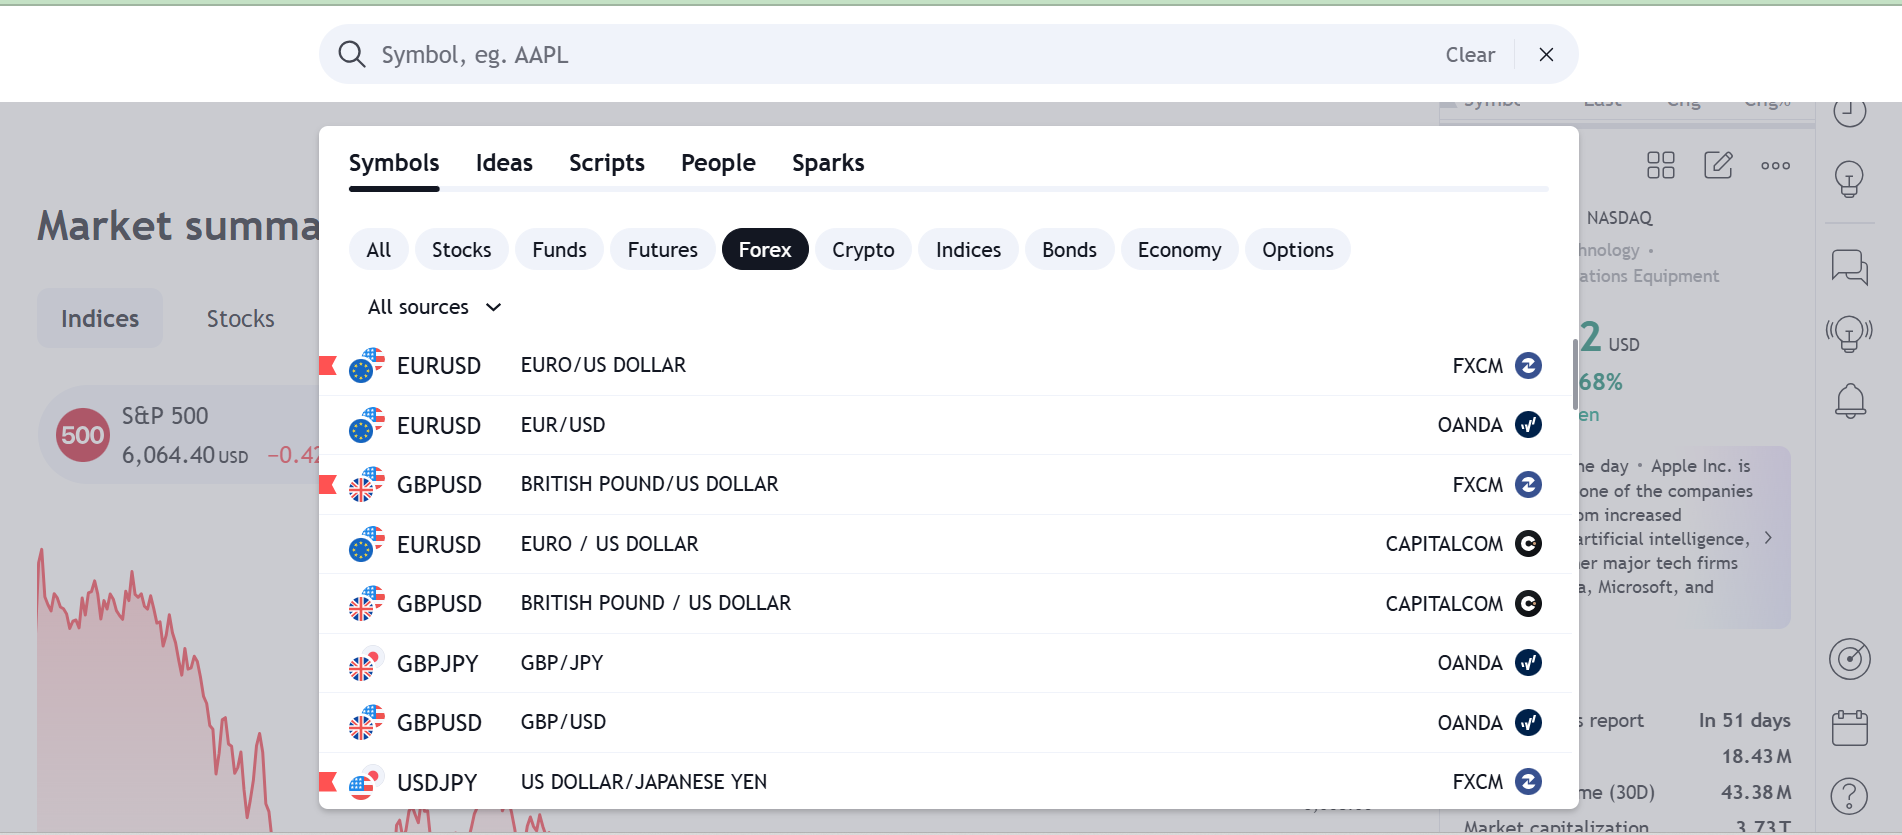
\includegraphics[scale=0.4]{gambar/gambarpasarmodalbeneran.png} 
    \caption{Overview Pasar Modal}
    \label{fig:label_gambar}
\end{figure}

\begin{figure} [H] \centering
  % Nama dari file gambar yang diinputkan
  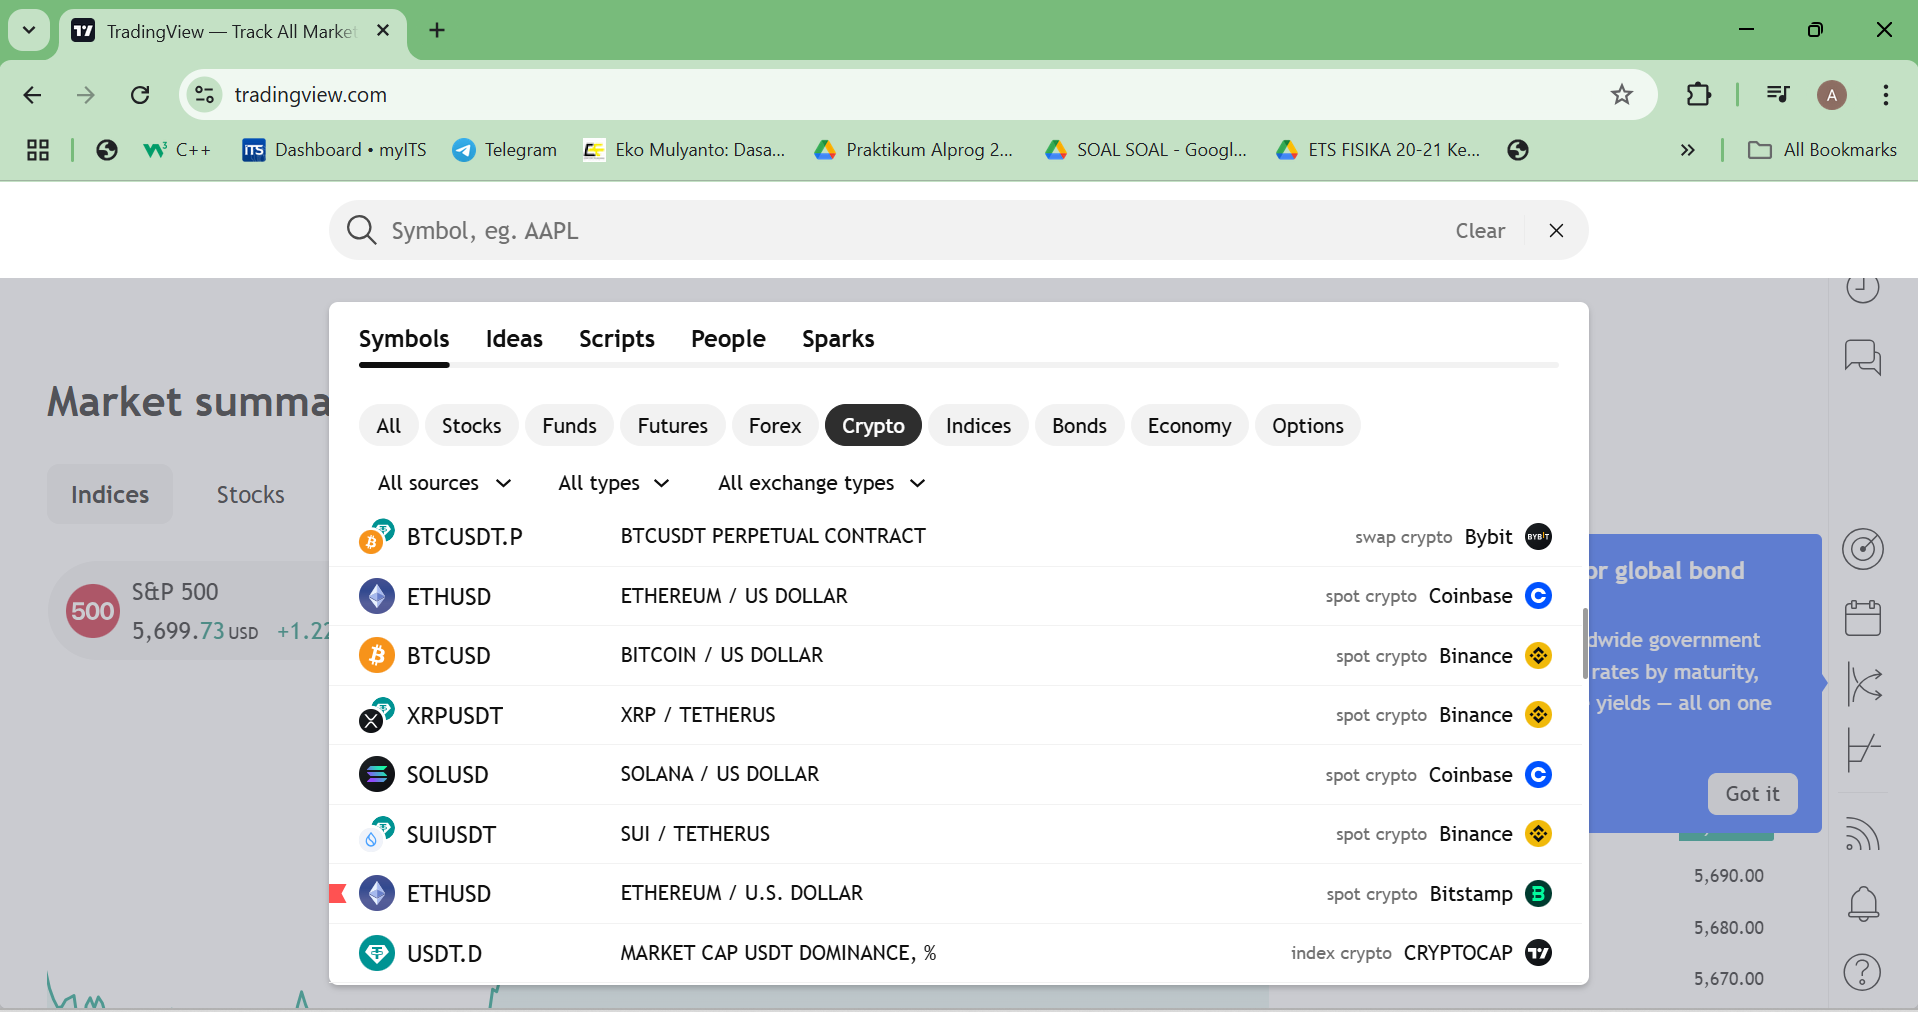
\includegraphics[scale=0.25]{gambar/CRYPTO.png} 
    \caption{Overview Pasar Modal}
    \label{fig:label_gambar}
\end{figure}

\begin{figure} [H] \centering
  % Nama dari file gambar yang diinputkan
  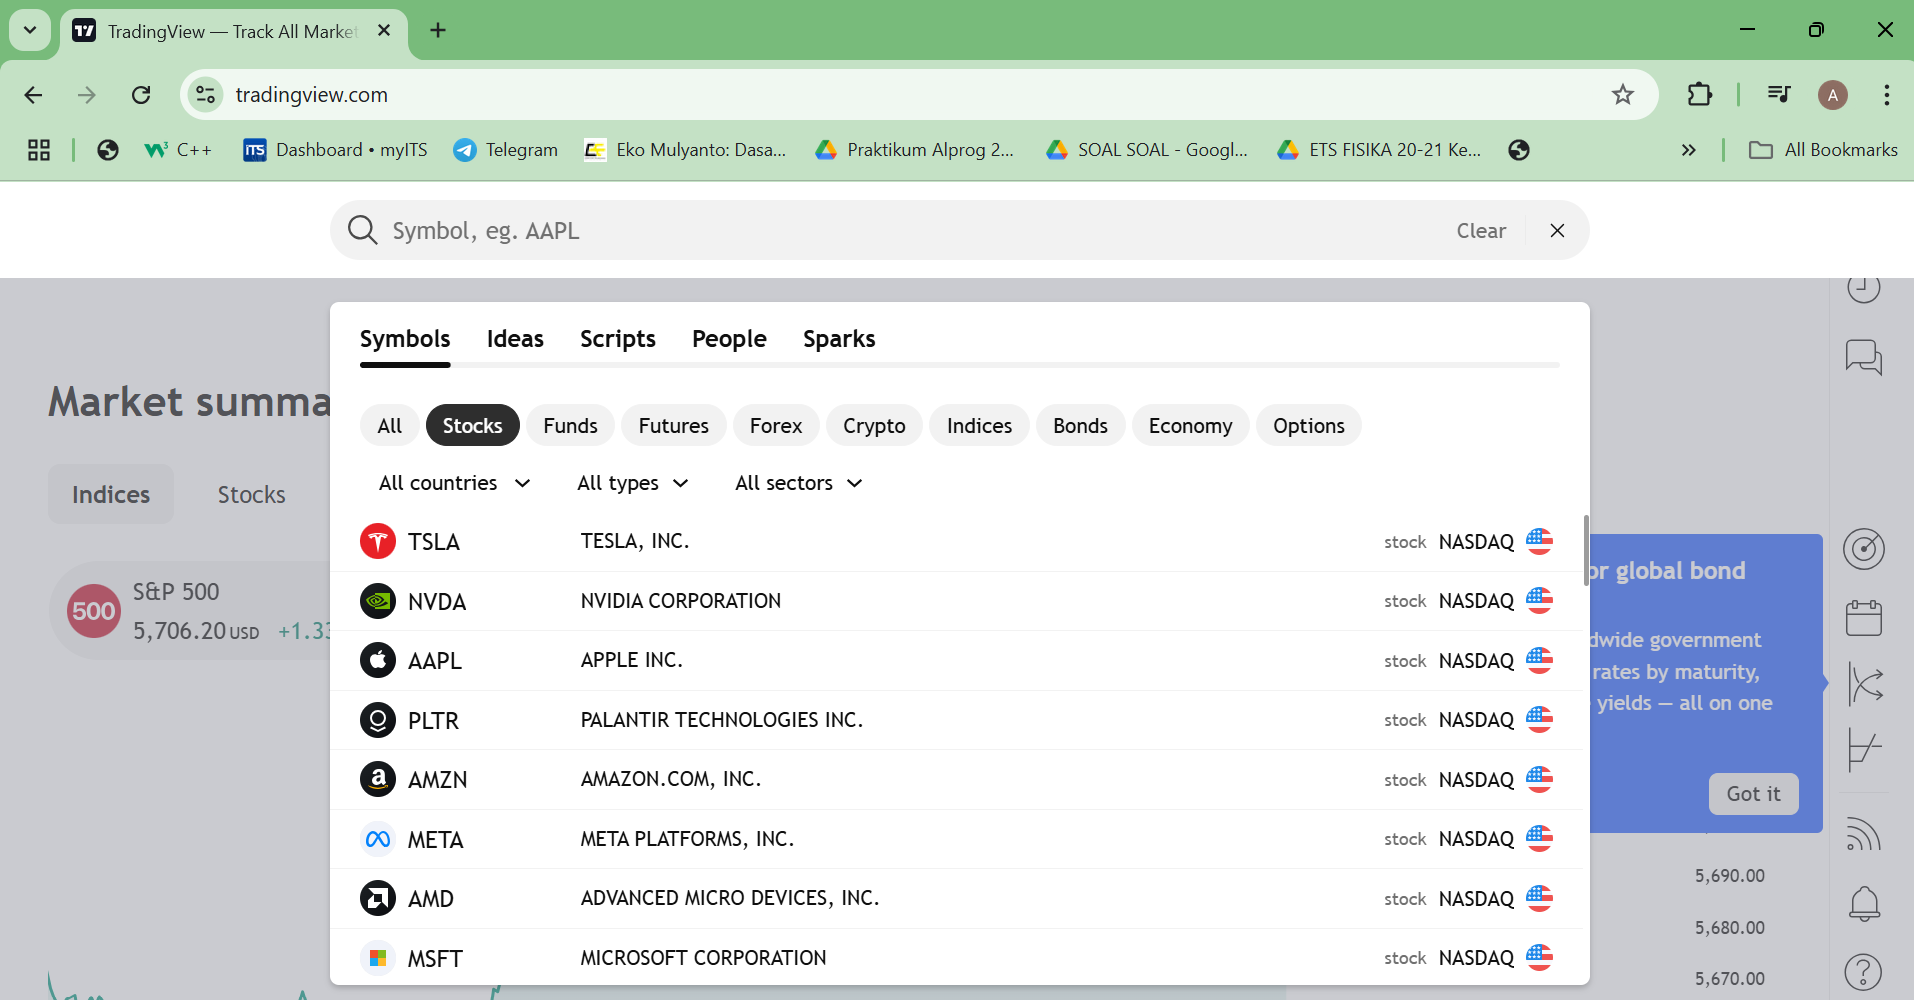
\includegraphics[scale=0.4]{gambar/STOCK.png} 
    \caption{Overview Pasar Modal}
    \label{fig:label_gambar}
\end{figure}
\subsubsection*{2.2.1.1 Pasar Forex}
Pasar Forex, atau pasar valuta asing, adalah pasar global di mana mata uang negara-negara di seluruh dunia diperdagangkan satu sama lain. Ini adalah pasar terbesar dan paling likuid di dunia, dengan volume transaksi harian mencapai lebih dari \$6 triliun pada 2023, menurut Bank for International Settlements (BIS)\autocite{bis2023triennial}. Pasar ini terbuka 24 jam sehari, lima hari seminggu, dan beroperasi tanpa lokasi fisik tunggal\autocite{hull2015options}. Sebagai pasar desentralisasi, forex berlangsung secara elektronik melalui berbagai platform dan sistem perdagangan yang menghubungkan bank, lembaga keuangan, pemerintah, perusahaan besar, dan trader individu.
\begin{enumerate}
    \item Fungsi Pasar Forex
    \begin{itemize}
        \item \textbf{Pertukaran Mata Uang untuk Perdagangan Internasional:} Perusahaan dan negara memerlukan mata uang asing untuk melakukan transaksi internasional. Misalnya, importir dan eksportir perlu membeli atau menjual mata uang asing untuk membayar barang dan jasa.
        \item \textbf{Manajemen Resiko (\textit{Hedging}):} Perusahaan dan investor menggunakan pasar forex untuk melindungi diri dari risiko perubahan nilai tukar yang dapat mempengaruhi pendapatan mereka. Misalnya, sebuah perusahaan yang memiliki eksposur terhadap mata uang asing akan melakukan kontrak derivatif untuk mengurangi potensi kerugian.
        \item \textbf{Spekulasi:}Trader individu dan lembaga keuangan sering berpartisipasi dalam pasar forex untuk meraih keuntungan dengan memprediksi pergerakan harga mata uang. Ini adalah salah satu aktivitas paling populer di pasar forex.
    \end{itemize}
    \item Pasangan Mata Uang (Currency Pairs)
    
    Di pasar forex, mata uang diperdagangkan dalam pasangan. Sebagai contoh, pasangan mata uang seperti EUR/USD (Euro terhadap Dolar AS) atau GBP/JPY (Pound Inggris terhadap Yen Jepang). Setiap pasangan mata uang terdiri dari:
    \begin{itemize}
        \item \textbf{Base Currency (Mata Uang Dasar):} Mata uang pertama dalam pasangan, misalnya Euro (EUR) dalam pasangan EUR/USD.
        \item \textbf{Quote Currency (Mata Uang Kuotasi):} Mata uang kedua dalam pasangan, misalnya Dolar AS (USD) dalam pasangan EUR/USD.
    \end{itemize}
    
    \item Satuan Pergerakan mata uang
    
    Dalam perdagangan forex \textit{(foreign exchange)}, istilah pips atau \textit{"percentage in point"} adalah satuan terkecil perubahan harga mata uang yang diperdagangkan di pasar valuta asing. Pips berfungsi sebagai pengukur pergerakan harga dan menjadi standar bagi para trader untuk menghitung keuntungan dan kerugian dalam transaksi.
    Secara umum, satu pip biasanya setara dengan pergerakan angka desimal keempat dalam pasangan mata uang dengan format empat desimal, misalnya:
    \begin{itemize}
        \item Jika EUR/USD bergerak dari 1.1000 ke 1.1001, maka perubahannya adalah 1 pip.
        \item Untuk pasangan mata uang tertentu seperti USD/JPY, pip dihitung pada angka desimal kedua, misalnya dari 110.00 ke 110.01 berarti 1 pip.
    \end{itemize}
\end{enumerate}
Perdagangan forex dilakukan melalui platform online, dan harga pasangan mata uang dipengaruhi oleh berbagai faktor ekonomi dan politik, termasuk:
Suku bunga, Kebijakan moneter dari bank sentral, tingkat pengangguran, inflasi.Pasar forex sangat volatil dan bisa sangat cepat bergerak. Oleh karena itu, prediksi harga di pasar forex memerlukan teknik analisis yang kuat dan cermat.
\begin{figure} [H] \centering
  % Nama dari file gambar yang diinputkan
  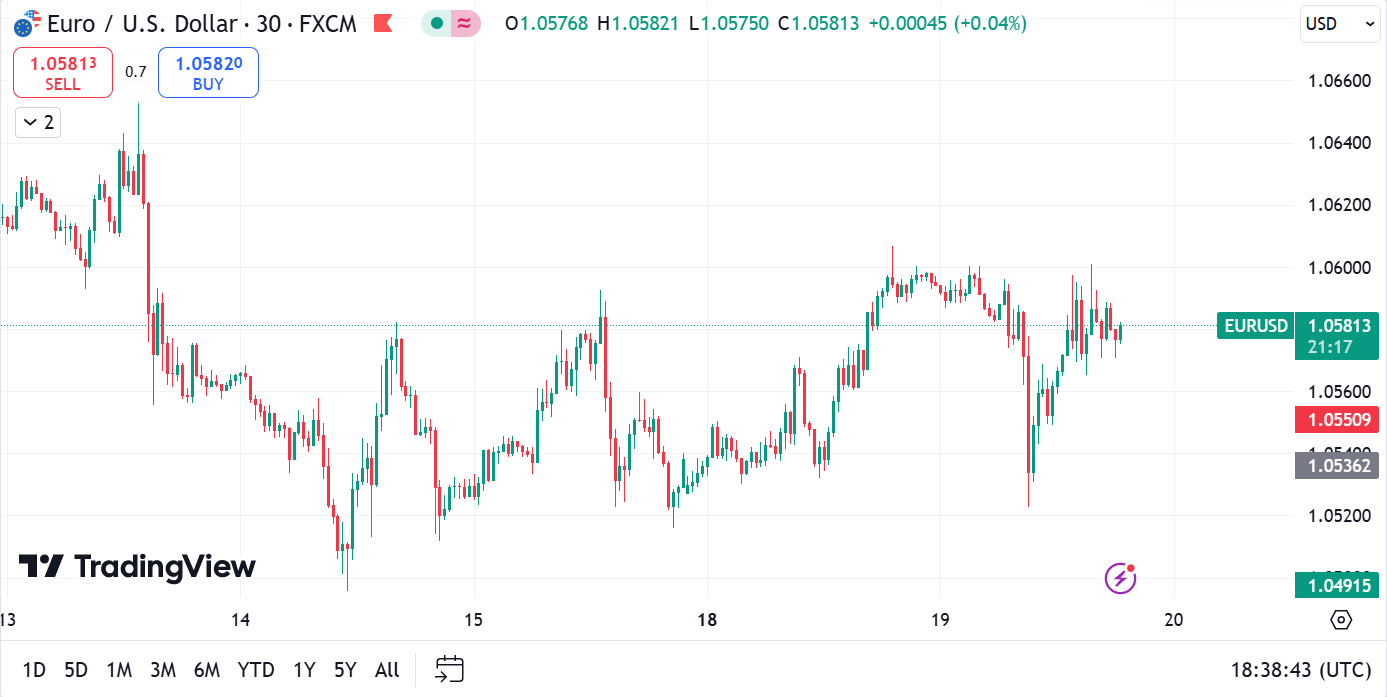
\includegraphics[scale=0.5]{gambar/gambarpasarmodal.png} 
    \caption{Overview forex usd/chf.}
    \label{fig:label_gambar}
\end{figure}

\subsection{Candlestick}
Candlestick adalah salah satu jenis grafik yang digunakan untuk menggambarkan pergerakan harga dalam pasar keuangan, seperti saham, forex, atau komoditas, dalam periode waktu tertentu. Setiap candlestick mewakili informasi tentang harga buka, harga tertinggi, harga terendah, dan harga tutup dalam satu periode waktu tertentu, misalnya per menit, jam, atau hari.

\begin{enumerate}
    \item Struktur Candlestick
    \begin{itemize}
        \item Body (Badan): Bagian tengah candlestick yang menggambarkan perbedaan antara harga buka dan harga tutup pada periode tersebut.
        \item Jika harga tutup lebih tinggi dari harga buka, body candlestick biasanya berwarna hijau atau putih, menandakan tren naik.
        \item Jika harga tutup lebih rendah dari harga buka, body candlestick biasanya berwarna merah atau hitam, menandakan tren turun.
        \item Wick (Sumbu): Garis vertikal yang terletak di atas dan di bawah body, yang menunjukkan harga tertinggi dan terendah dalam periode waktu tersebut.
        \item Upper Wick (Sumbu Atas): Menunjukkan perbedaan antara harga tertinggi dan harga buka (untuk candlestick bullish) atau harga tertinggi dan harga tutup (untuk candlestick bearish).
        \item Lower Wick (Sumbu Bawah): Menunjukkan perbedaan antara harga terendah dan harga buka (untuk candlestick bullish) atau harga terendah dan harga tutup (untuk candlestick bearish).

    \end{itemize}
    \item Elemen Candlestick
    \begin{itemize}
        \item Harga Buka: Harga pada awal periode waktu.
        \item Harga Tutup: Harga pada akhir periode waktu.
        \item Harga Tertinggi: Harga tertinggi yang tercatat selama periode tersebut.
        \item Harga Terendah: Harga terendah yang tercatat selama periode tersebut.
    \end{itemize}
    \item Jenis-Jenis Candlestick
    \begin{itemize}
        \item Bullish Candlestick (Kenaikan Harga): Body candlestick terbentuk dengan harga tutup yang lebih tinggi daripada harga buka, dan umumnya berwarna hijau atau putih. Ini menandakan bahwa harga bergerak naik selama periode tersebut.
        \item Bearish Candlestick (Penurunan Harga): Body candlestick terbentuk dengan harga tutup yang lebih rendah daripada harga buka, dan biasanya berwarna merah atau hitam. Ini menandakan bahwa harga bergerak turun selama periode tersebut.
    \end{itemize}
\end{enumerate}
\begin{figure} [H] \centering
  % Nama dari file gambar yang diinputkan
    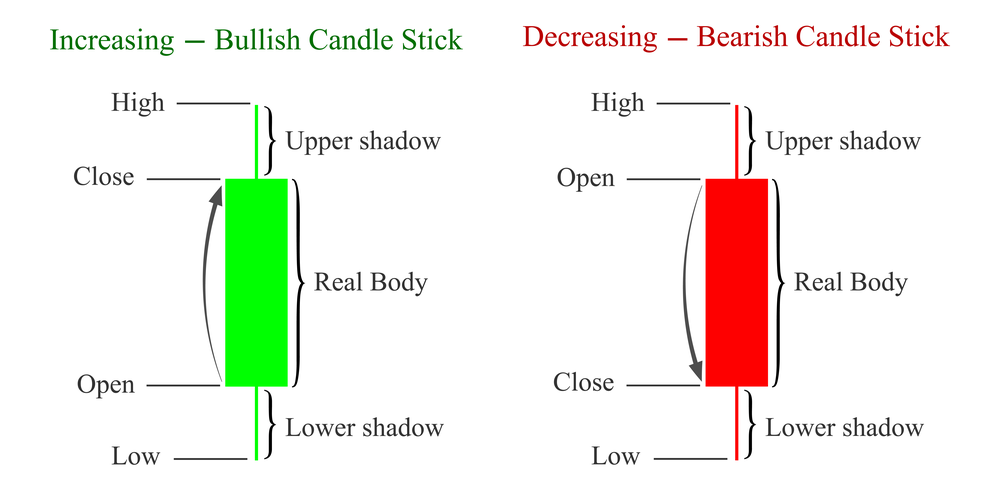
\includegraphics[scale=1.4]{gambar/candlestick.png} 
    \caption{CandleStick}
    \label{fig:label_gambar}
\end{figure}

\subsection{Broker}
Dalam aktivitas perdagangan valuta asing (foreign exchange/forex), broker forex merupakan pihak atau perusahaan yang bertindak sebagai perantara antara trader individu maupun institusi dengan pasar valuta asing global. Pasar forex sendiri merupakan pasar keuangan terbesar di dunia yang bersifat desentralisasi dan beroperasi secara over-the-counter (OTC), sehingga transaksi antar pelaku pasar dilakukan secara langsung melalui jaringan elektronik tanpa adanya bursa terpusat. Dalam hal ini, broker forex menjadi fasilitator yang menyediakan akses bagi trader untuk melakukan transaksi jual beli pasangan mata uang melalui platform trading yang disediakan.

Menurut Babypips (n.d.), broker forex berperan penting karena pasar forex umumnya didominasi oleh institusi keuangan besar, bank sentral, hedge fund, dan perusahaan multinasional. Tanpa adanya broker forex, trader individu tidak memiliki akses langsung ke pasar antar bank tempat transaksi mata uang dalam volume besar dilakukan. Broker forex memberikan berbagai layanan mulai dari penyediaan data harga pasar secara real-time, eksekusi order transaksi, hingga fasilitas manajemen risiko bagi para trader.

Fungsi dan Layanan Broker Forex
Secara umum, fungsi utama broker forex meliputi beberapa hal berikut:
\begin{enumerate}
    \item \textbf{Menyediakan Platform Perdagangan}
    
    Broker forex menyediakan platform trading berbasis desktop maupun mobile, seperti MetaTrader 4 (MT4), MetaTrader 5 (MT5), atau aplikasi berbasis web. Melalui platform ini, trader dapat melakukan analisis harga, eksekusi order, serta pemantauan posisi transaksi secara real-time.
    
    \item \textbf{Memberikan Fasilitas Leverage}

    Broker forex biasanya menawarkan fasilitas leverage, yaitu pinjaman modal dari broker kepada trader agar dapat melakukan transaksi dengan nilai kontrak yang lebih besar dibandingkan dengan modal yang dimiliki. Sebagai contoh, leverage 1:100 memungkinkan trader dengan modal \$100 untuk melakukan transaksi senilai \$10.000. Namun, penggunaan leverage juga meningkatkan potensi risiko kerugian.

    \item \textbf{Menyediakan Harga Pasar dan Spread}

    Broker bertanggung jawab menyediakan harga bid (jual) dan ask (beli) untuk setiap pasangan mata uang. Perbedaan antara harga bid dan ask disebut spread, yang menjadi sumber keuntungan utama bagi broker forex, terutama broker dengan tipe dealing desk.

    \item \textbf{Memberikan Fasilitas Manajemen Risiko}

    Broker forex menyediakan berbagai fitur manajemen risiko seperti \textbf{stop loss, take profit, margin call, dan negative balance protection} untuk membantu trader mengendalikan risiko kerugian dalam aktivitas perdagangan.

    \item \textbf{Penyediaan Edukasi dan Analisis Pasar}

    Banyak broker forex juga menawarkan fasilitas edukasi bagi trader pemula maupun profesional, berupa artikel, video tutorial, webinar, serta analisis pasar harian atau mingguan.

    \item \textbf{Penyediaan Akun Demo}

    Broker forex umumnya menyediakan akun demo yang memungkinkan trader berlatih melakukan transaksi di lingkungan pasar simulasi dengan data harga real-time, tanpa menggunakan dana sungguhan.
\end{enumerate}

Proses kerja broker forex dimulai ketika trader membuka akun trading di broker tertentu, kemudian menyetorkan dana sebagai modal transaksi. Melalui platform trading yang disediakan, trader dapat melakukan analisis pasar dan menempatkan order beli atau jual pasangan mata uang. Broker akan meneruskan order tersebut ke penyedia likuiditas atau pasar antar bank sesuai dengan tipe broker yang digunakan.

Setiap transaksi trader akan dikenakan biaya berupa spread atau komisi sesuai kebijakan broker. Selain itu, broker juga menyediakan fasilitas leverage dan margin yang memungkinkan trader mengendalikan nilai kontrak transaksi dalam jumlah besar, meskipun hanya dengan modal relatif kecil. Broker forex juga bertugas melakukan eksekusi order secara cepat dan akurat agar transaksi dapat terjadi sesuai harga yang diinginkan trader.

Broker forex memiliki peran strategis dalam memastikan kelancaran aktivitas perdagangan valuta asing, khususnya bagi trader individu yang tidak memiliki akses langsung ke pasar antar bank. Selain sebagai perantara transaksi, broker juga berperan sebagai penyedia fasilitas edukasi, informasi pasar, dan teknologi trading. Ketersediaan broker forex yang andal dan teregulasi menjadi faktor penting dalam menciptakan ekosistem perdagangan yang aman, transparan, dan efisien.

\subsection{Analisis Teknikal}
Analisis teknikal adalah metode analisis pasar yang memanfaatkan data historis harga dan volume perdagangan untuk memprediksi pergerakan harga di masa depan. Dalam praktiknya, analisis teknikal lebih menitikberatkan pada pergerakan harga (\textit{price action}) dan pola-pola grafik (\textit{chart patterns}) dibandingkan dengan faktor-faktor fundamental seperti kondisi ekonomi, politik, atau kinerja perusahaan.Analisis teknikal didasarkan pada tiga asumsi utama:

\begin{enumerate}
    \item Harga yang tercatat di pasar sudah mencerminkan semua informasi yang tersedia, baik ekonomi, politik, maupun faktor psikologis.

    \item Pergerakan harga cenderung mengikuti suatu tren, baik itu tren naik (\textit{uptrend}), tren turun (\textit{downtrend}), atau bergerak dalam kisaran tertentu (\textit{sideways}). Prinsip ini menyatakan bahwa tren harga akan berlanjut sampai ada sinyal pembalikan yang jelas.

    \item Pola pergerakan harga cenderung berulang karena faktor psikologi pasar dan perilaku pelaku pasar dari waktu ke waktu. Oleh sebab itu, pola-pola grafik yang muncul di masa lalu dapat digunakan sebagai acuan untuk memprediksi pergerakan harga berikutnya.
\end{enumerate}

Berikut merupakan beberapa teknikal analisis yang biasa digunakan para pelaku pasar modal untuk menganalisis chart pada forex:

\subsubsection*{2.2.4.1 Head \& Shoulders}
Head and Shoulders adalah salah satu pola chart pattern dalam analisis teknikal yang digunakan untuk mengidentifikasi potensi pembalikan arah tren harga di pasar, termasuk dalam pasar forex. Pola ini dianggap sebagai salah satu pola pembalikan (\textit{reversal pattern}) yang paling andal oleh para trader teknikal.

Pola ini dinamakan Head and Shoulders karena bentuknya menyerupai bahu kiri (\textit{left shoulder}), kepala (\textit{head}), dan bahu kanan (\textit{right shoulder}). Secara visual, pola ini terbentuk ketika harga menunjukkan tiga puncak, di mana:

\begin{enumerate}
    \item \textbf{Left Shoulder}: Harga naik ke puncak dan kemudian turun.
    \item \textbf{Head}: Harga kembali naik ke puncak yang lebih tinggi dari puncak sebelumnya, lalu turun lagi.
    \item \textbf{Right Shoulder}: Harga naik lagi, tetapi hanya mencapai puncak yang lebih rendah daripada kepala, lalu turun kembali.
\end{enumerate}

\begin{figure} [H] \centering
  % Nama dari file gambar yang diinputkan
    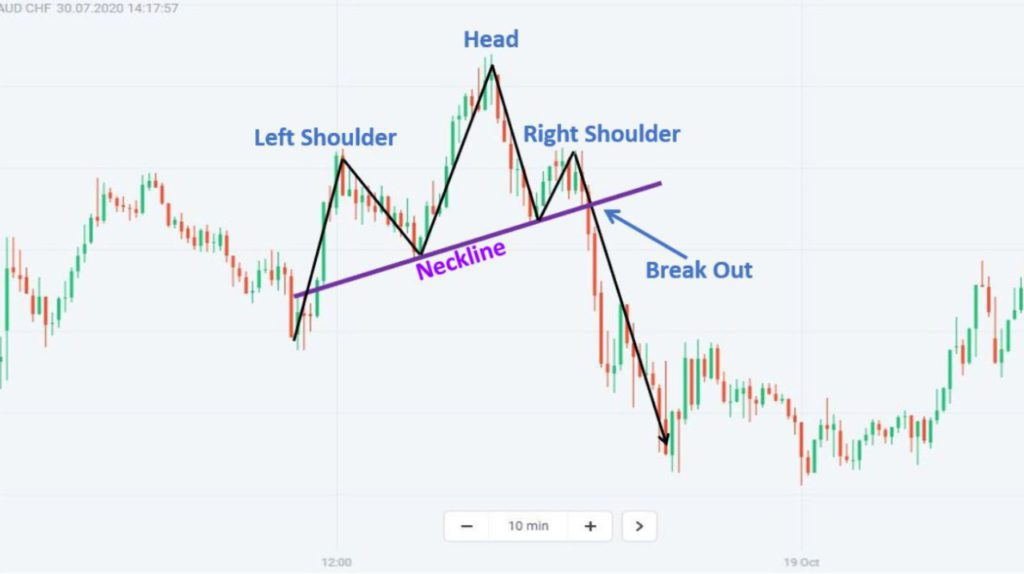
\includegraphics[scale=0.35]{gambar/headshoulders.jpg} 
    \caption{Head \& Shoulders Chart Pattern}
    \label{fig:label_gambar}
\end{figure}

Penurunan setelah bahu kanan biasanya menembus garis leher (\textit{neckline}), yang merupakan garis support yang menghubungkan titik terendah antara head dan kedua shoulders. \textit{Breakout} dari \textit{neckline} ini sering dijadikan sinyal kuat bahwa tren akan berbalik arah.

\subsubsection*{2.2.4.2 Double Top}
Double Top adalah salah satu pola chart pattern dalam analisis teknikal yang menunjukkan potensi pembalikan arah tren (\textit{trend reversal}) dari tren naik menjadi tren turun. Pola ini terbentuk ketika harga mencapai \textit{level resistance} yang sama sebanyak dua kali, namun gagal menembusnya dan kemudian mengalami penurunan.Pola ini banyak digunakan oleh trader forex untuk mengidentifikasi area potensial di mana harga diperkirakan akan mengalami koreksi atau pembalikan tren setelah tren naik.
\begin{figure} [H] \centering
  % Nama dari file gambar yang diinputkan
    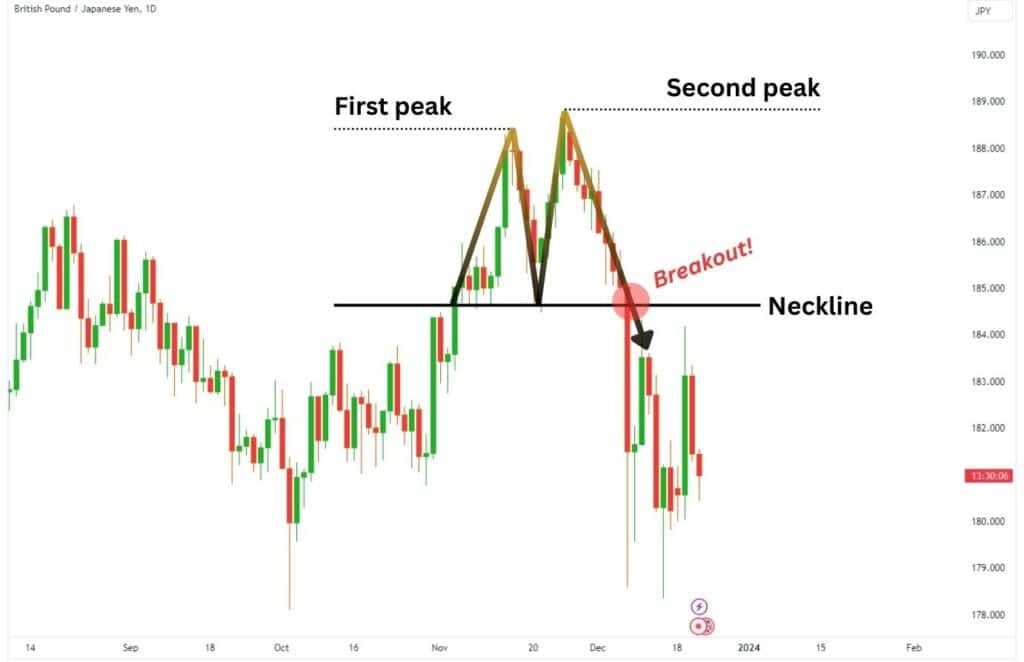
\includegraphics[scale=0.3]{gambar/doubletop.jpg} 
    \caption{Double Top Chart Pattern}
    \label{fig:label_gambar}
\end{figure}

Pola Double Top terdiri dari dua puncak harga (\textit{peak/top}) yang hampir setara ketinggiannya, dipisahkan oleh sebuah lembah (\textit{valley}) di antaranya. Setelah harga membentuk puncak kedua dan gagal menembus puncak pertama, harga biasanya turun ke bawah garis support yang dikenal dengan sebutan \textit{neckline}.

Jika harga berhasil menembus \textit{neckline} ke bawah, maka konfirmasi pola \textit{double top} dianggap valid dan mengindikasikan potensi pembalikan tren dari \textit{bullish} menjadi \textit{bearish}.


\subsection{Deep Learning }
Deep learning adalah cabang dari machine learning yang berfokus pada penggunaan jaringan saraf tiruan (Artificial Neural Networks) dengan banyak lapisan (multi-layered) untuk mempelajari representasi data yang kompleks. Konsep ini terinspirasi dari cara kerja otak manusia yang terdiri dari neuron-neuron yang saling terhubung untuk memproses informasi secara paralel\autocite{lecun2015deep}. Deep learning mulai berkembang pesat seiring dengan kemajuan teknologi komputasi, ketersediaan data dalam jumlah besar , serta peningkatan algoritma optimasi yang efektif. Keunggulan deep learning terletak pada kemampuannya dalam menangkap pola-pola non-linear, mengenali fitur kompleks dari data, serta memproses data dengan dimensi yang tinggi\autocite{goodfellow2016deep}.

Keunggulan utama Transformer terletak pada kemampuan pemrosesan paralel yang signifikan, serta kemampuannya dalam menangkap pola jangka panjang dan dependensi kompleks dalam data\autocite{hochreiter1997long}. Selain itu, positional encoding ditambahkan untuk mempertahankan informasi urutan waktu pada data time series. Dalam prediksi harga pasar modal, arsitektur Time Series Transformer memanfaatkan kemampuan self-attention untuk menganalisis fluktuasi historis harga seperti Open, High, Low, dan Close (OHLC). Hal ini memungkinkan model mempelajari pola volatilitas pasar secara lebih akurat dan efisien. Dengan fleksibilitas input serta kemampuannya dalam memproses data berukuran besar, Time Series Transformer menjadi solusi yang efektif dalam meningkatkan akurasi prediksi pada data pasar modal.

\subsection{Deret Waktu \textit{(Time Series)}}
Deret waktu atau time series adalah serangkaian data yang dikumpulkan atau diukur secara berurutan berdasarkan waktu. Data ini memiliki karakteristik penting yaitu dependensi temporal, di mana nilai pada waktu tertentu bergantung pada nilai-nilai sebelumnya atau masa lalu. Analisis deret waktu bertujuan untuk memahami pola historis dari data dan melakukan prediksi terhadap nilai di masa depan\autocite{box2015time}. Deret waktu sering digunakan dalam berbagai bidang seperti ekonomi, keuangan, cuaca, dan industri untuk memprediksi tren dan fluktuasi. Dalam konteks pasar modal, data deret waktu terdiri dari informasi historis seperti harga Open, High, Low, dan Close (OHLC) yang memiliki sifat dinamis dan volatil, serta sangat dipengaruhi oleh faktor internal maupun eksternal.

Metode tradisional seperti MA (Moving Average) telah lama digunakan untuk analisis deret waktu karena kemampuannya menangkap pola linear dalam data. Namun, metode ini memiliki keterbatasan dalam memodelkan pola yang non-linear dan kompleks, serta kesulitan dalam menangkap dependensi jangka panjang. Kelemahan ini mendorong penggunaan metode berbasis deep learning seperti Recurrent Neural Networks (RNN) dan Long Short-Term Memory (LSTM), yang dirancang khusus untuk menangani data sekuensial. LSTM memperbaiki kelemahan RNN dengan mekanisme gates yang memungkinkan model menangkap hubungan temporal jangka pendek maupun jangka panjang secara lebih efektif. Meski begitu, LSTM masih memiliki tantangan dalam efisiensi komputasi karena proses pelatihan yang bersifat berurutan (sequential).

Untuk mengatasi keterbatasan tersebut, arsitektur Transformer dikembangkan sebagai solusi yang lebih efisien dan akurat dalam analisis deret waktu. Berbeda dengan RNN dan LSTM, Transformer menggunakan self-attention mechanism untuk mempelajari hubungan temporal di seluruh titik waktu secara paralel, sehingga memungkinkan pemrosesan yang lebih cepat dan efektif. Dengan positional encoding, Transformer tetap dapat mempertahankan informasi urutan waktu dalam data time series. Pada prediksi harga pasar modal, pendekatan ini memungkinkan model untuk menangkap pola fluktuasi harga dengan lebih baik, termasuk interaksi kompleks antar variabel seperti harga Open, High, Low, dan Close. Dengan demikian, penggunaan Time Series Transformer menjadi pendekatan yang unggul dalam analisis dan prediksi deret waktu karena mampu memodelkan dependensi temporal jangka panjang, menangani non-linearitas data, serta meningkatkan efisiensi komputasi dalam proses pelatihan. 

Dalam prediksi harga pasar modal, data deret waktu sering digunakan untuk menangkap pola musiman, siklus, atau tren jangka panjang.Komponen utama deret waktu adalah
\begin{enumerate}
    \item Trend: Komponen deret waktu yang menggambarkan pola perubahan jangka panjang dalam data. Trend menunjukkan arah umum pergerakan data, apakah naik, turun, atau tetap stabil selama periode waktu tertentu. Misalnya, jika penjualan suatu produk terus meningkat selama beberapa tahun, maka ada trend naik pada data penjualan tersebut.
    \begin{figure} [H] \centering
    % Nama dari file gambar yang diinputkan
    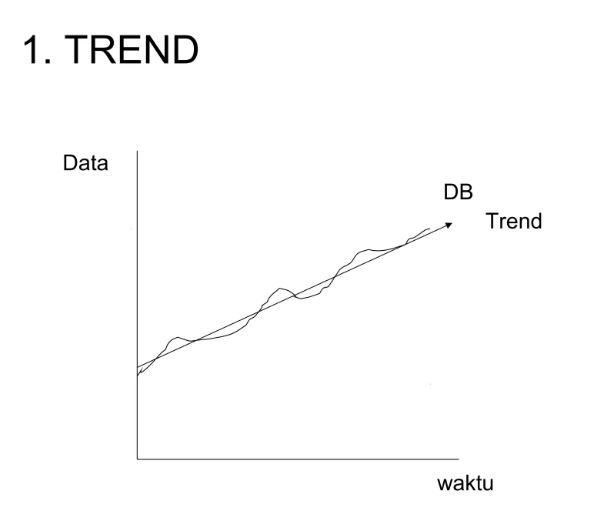
\includegraphics[scale=0.8]{gambar/deret waktu trend.png} 
    \caption{Pola Trend}
    \label{fig:label_gambar}
    \end{figure}
    \item Musiman (Seasonality): Fluktuasi teratur dalam data yang terjadi pada interval waktu tertentu, biasanya dalam siklus yang berulang secara tahunan, bulanan, atau mingguan. Komponen musiman mencerminkan pola yang terjadi pada waktu tertentu dalam setahun atau bulan tertentu.Pola berulang berdasarkan waktu, seperti kuartal atau tahun.
    \begin{figure} [H] \centering
     % Nama dari file gambar yang diinputkan
    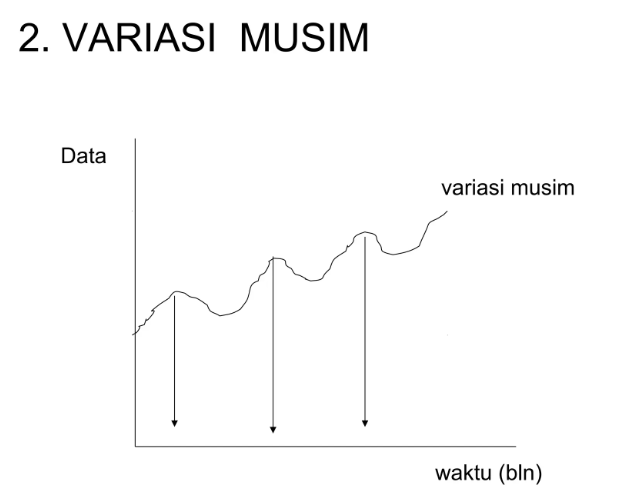
\includegraphics[scale=0.8]{gambar/deret waktu musiman.png} 
    \caption{Pola Musiman.}
    \label{fig:label_gambar}
    \end{figure}
    \item Noise: Noise merujuk pada fluktuasi atau gangguan acak dalam data yang tidak dapat dijelaskan oleh komponen trend atau musiman. Noise adalah variabilitas yang tidak teratur dan tidak dapat diprediksi dalam data. Ini sering kali disebabkan oleh faktor eksternal yang tidak terkontrol, kesalahan pengukuran, atau faktor lain yang tidak terkait dengan pola jangka panjang atau musiman. Noise sering dianggap sebagai "gangguan" dalam analisis deret waktu, karena sulit untuk diprediksi atau dimodelkan secara langsung.
    \begin{figure} [H] \centering
     % Nama dari file gambar yang diinputkan
    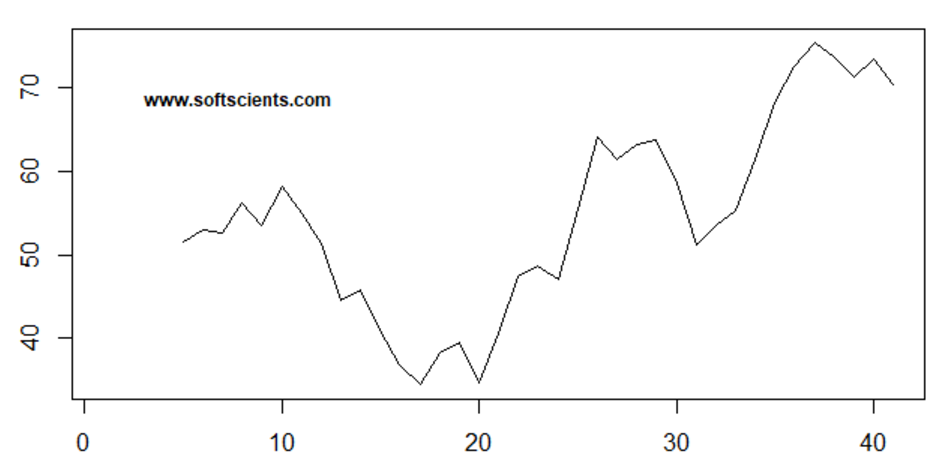
\includegraphics[scale=0.8]{gambar/deret waktu noise.png} 
    \caption{Pola Noise.}
    \label{fig:label_gambar}
\end{figure}
\end{enumerate}

\subsection{Time Series Transformer \textit{(TST)}}
Time Series Transformer adalah model deep learning yang dikembangkan berdasarkan arsitektur Transformer yang pertama kali diperkenalkan oleh Vaswani et al. (2017) dalam paper "Attention Is All You Need". Transformer dirancang untuk menangani data sekuensial dengan pendekatan self-attention mechanism, yang memungkinkan model untuk mempelajari hubungan antara elemen dalam urutan data secara paralel dan efisien. Berbeda dengan metode tradisional seperti ARIMA atau model berbasis Recurrent Neural Networks (RNN) dan Long Short-Term Memory (LSTM), Transformer tidak memproses data secara sequential melainkan menggunakan mekanisme perhatian untuk mengidentifikasi dependensi jangka pendek maupun jangka panjang dalam data\autocite{hochreiter1997long}. Hal ini membuat Transformer unggul dalam menangani long-term dependencies dan non-linear relationships yang sering muncul pada data time series, termasuk prediksi harga pasar modal.

Pada model Time Series Transformer, komponen self-attention memainkan peran utama dalam mengidentifikasi kontribusi dari setiap titik waktu terhadap prediksi masa depan. Mekanisme ini bekerja dengan menghitung bobot perhatian antara setiap titik waktu dalam data input, di mana nilai perhatian yang lebih besar diberikan pada titik-titik yang dianggap lebih relevan\autocite{vaswani2017attention}. Untuk mempertahankan informasi urutan waktu, Time Series Transformer menggunakan positional encoding, yang menambahkan informasi posisi ke dalam representasi data sebelum diolah oleh model. Dengan ini, model dapat memahami konteks temporal dari data time series meskipun pemrosesan dilakukan secara paralel.

Dalam konteks prediksi harga pasar modal, Time Series Transformer digunakan untuk menganalisis data historis seperti harga Open, High, Low, dan Close (OHLC). Kemampuan model ini untuk mempelajari pola volatilitas yang kompleks serta menangkap hubungan temporal antar variabel memungkinkan prediksi yang lebih akurat dibandingkan metode konvensional\autocite{goodfellow2016deep}. Selain itu, fleksibilitas arsitektur Transformer memudahkan integrasi dengan berbagai fitur tambahan, seperti indikator teknikal atau data ekonomi makro, yang sering digunakan dalam analisis pasar. Dengan efisiensi komputasi dan performa yang unggul dalam menangkap pola kompleks, Time Series Transformer menjadi pendekatan yang sangat cocok untuk prediksi harga pasar modal dalam skenario data berskala besar.



Komponen Utama Time Series Transformer
\begin{enumerate}
    \item Attention Mechanism:
    \begin{itemize}
        \item Mengidentifikasi hubungan antara titik-titik data deret waktu secara global, sehingga mampu menangkap pola jangka panjang dan interaksi antarvariabel.
        \item Dua varian populer: Self-Attention dan Multi-Head Attention.
    \end{itemize}
    \item Positional Encoding:
    \begin{itemize}
        \item Karena Transformer tidak memiliki pemahaman urutan data bawaan, informasi posisi ditambahkan untuk menjaga konteks urutan waktu.
    \end{itemize}
    \item Encoder-Decoder Architecture:
     \begin{itemize}
        \item Encoder: Memahami pola historis dari data input.
        \item Decoder: Menghasilkan prediksi untuk langkah waktu berikutnya.
    \end{itemize}
    
\end{enumerate}
% Contoh penggunaan referensi dari persamaan
Time Series Transformer mempunyai arsitektur sebagai berikut.
\begin{figure} [H] \centering
  % Nama dari file gambar yang diinputkan
  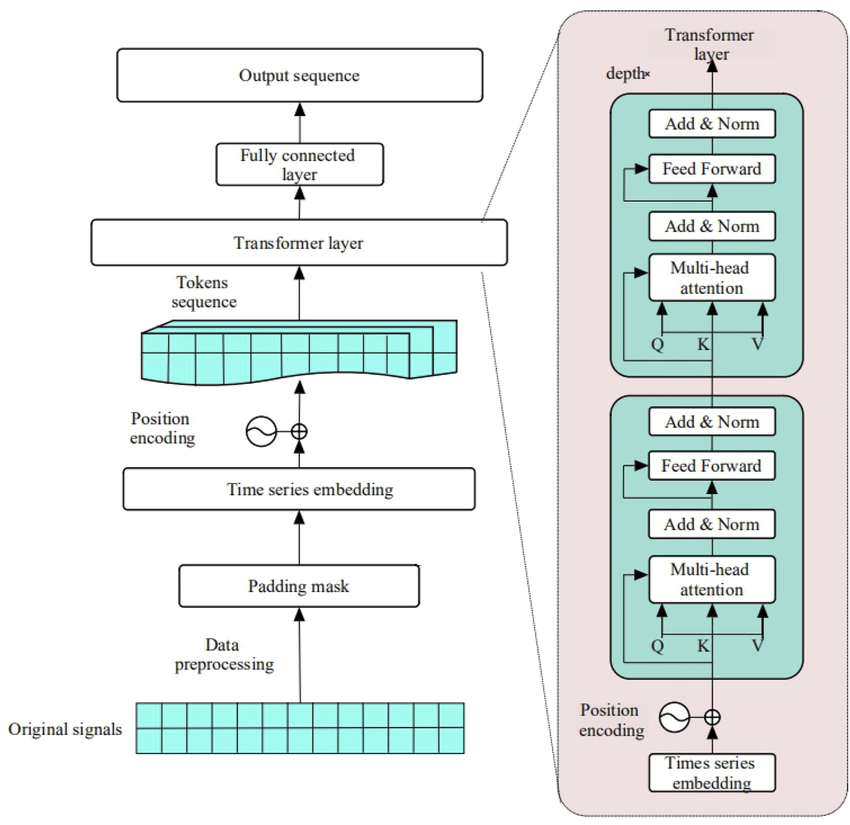
\includegraphics[scale=1.2]{gambar/gambar TST.png} 
    \caption{Arsitektur Time Series Transformer.}
    \label{fig:label_gambar}
\end{figure}
\begin{enumerate}
    \item \textbf{Data Prepocessing \& Embedding:} dalam lapisan ini terdapat beberapa langkah yang akan dilakukan. Data akan dinormalisasikan dengan cara membagi data menjadi skala yang lebih kecil menggunakan min-max scalling, dan padding digunakan untuk memastikan bahwa semua input memiliki panjang yang sama untuk membantu model memahami perbedaan antar fitur.Setelah itu akan ditambahkan keterangan waktu seperti menit jam atau hari untuk membantu model menangkap pola dari data. menginput dataset deret waktu multivarian dan memberikan input urutan waktu yang benar.
    \item \textbf{Transformer layer:} Lapisan ini akan memulai untuk mengolah data yang telah disiapkan di tahap selanjutnya,inti dari transformer adalah \textit{Self-attention} yang memungkinkan model untuk memahami hubungan antar eleman di dalam data.Layer ini akan mempelajari dan  menangkap hubungan temporal time series dari data, dan juga menggunakan beberapa kepala\textit{(heads)} untuk menangkap berbagai jenis hubungan temporal dalam data.Berikut adalah formula yang dipakai untuk \textit{Multi-Head Attention}
   \item \textbf{Output layer:} Lapisan output dalam Time Series Transformer bertugas untuk mengubah representasi terakhir dari encoder dan decoder untuk menjadi prediksi yang sesuai dari dataset yang telah diberikan. Lapisan ini sangat penting karena menentukan bagaimana model mengolah dan mempelajari informasi yang telah diberikan dan mengeluarkan hasil yang dapat digunakan.

\end{enumerate}

\cleardoublepage

% Bab 3 desain dan implementasi
\chapter{DESAIN DAN IMPLEMENTASI}
\label{chap:desainimplementasi}

% Ubah konten-konten berikut sesuai dengan isi dari metodologi
Pada bab ini akan dijelaskan mengenai bagaimana langkah langkah yang akan dilakukan sehinggga mendapatkan hasil yang diinginkan. Sistem ini bertujuan untuk membuat model yang dapat memprediksi harga pasar modal menggunakan model Time Series Transformer sebagai alat yang akan mempelajari data time series yang akan diinput dan bagaimana performa dari model tersebut.
\section{Metode yang digunakan}


\begin{figure} [H] \centering
  % Nama dari file gambar yang diinputkan
  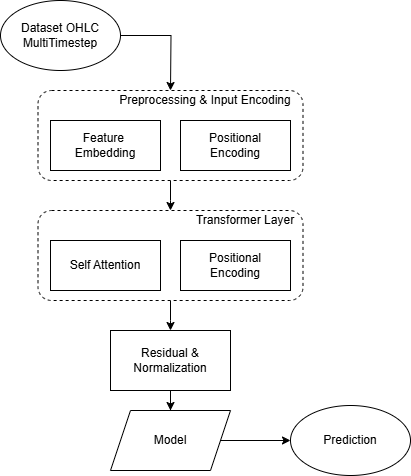
\includegraphics[scale=0.7]{gambar/diagram_abel.png} 
    \caption{Diagram Alur Model}
    \label{fig:diagram_abel}
\end{figure}


Pada \emph{Diagram} yang tertera di \ref{fig:diagram_abel}. Akan digunakan metode seperti berikut: 

\newpage
\section{Pengumpulan Dataset}
Pengumpulan dataset merupakan tahap awal dalam proses pembangunan model Time Series Transformer. Data yang didapatkan bersumber dari broker MT4.
Data yang digunakan terdiri dari data harga open, close, high, low,serta volume perdagangan. Dataset dapat diperoleh dari berbagai sumber terpercaya seperti situs web keuangan atau aplikasi penyedia data pasar modal yang menyediakan data historis dengan cakupan waktu tertentu. Dataset yang digunakan dalam penelitian ini dalam format CSV. Dalam penelitian ini penulis mendapat dataset tersebut dari platform yang bernama Meta Trader, salah satu platform untuk melakukan jual-beli pasar modal. Dataset yang digunakan merupakan data harga USD/CHF dengan waktu per 5 menit, merupakan daftar harga tukar US Dollar dan Franc Swiss dari 12 juli 2022 sampai 13 November 2023. 

\begin{figure} [H] \centering
  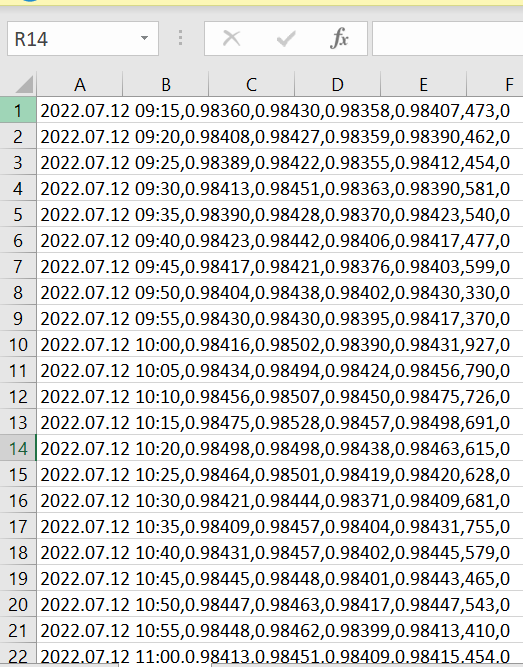
\includegraphics[scale=1.0]{gambar/gambar pengumpulan datset.png} 
    \caption{Dataset}
    \label{fig:dataset}
\end{figure}

Gambar \ref{fig:dataset} menunjukkan dataset yang digunakan dalam penelitian ini. Dataset ini berisi informasi harga pasar modal yang akan digunakan sebagai input untuk model Time Series Transformer dan model LSTM. Dataset ini berisi 100.001 data, dengan fitur yang terdiri dari tanggal, harga open, close, high, low, dan volume perdagangan. 

\section{Preprocessing \& Input Encoding}
Pada tahap ini,digunakan beberapa metode untuk menyiapkan dataset agar dapat digunakan sebagai dataset awal sebelum dilanjutkan ke transformer layer.


\subsection{\textbf{Feature Embedding}} Feature embedding adalah teknik untuk merepresentasikan fitur input dalam bentuk vektor berdimensi lebih rendah tetapi informatif. Dalam konteks Time Series Transformer, embedding bertujuan mengubah data numerik atau kategorikal menjadi representasi yang dapat diproses oleh model. Dari data yang diperoleh (\textit{Date,open,close,high,low,volume}), embedding dapat mengubah setiap fitur menjadi vektor dengan dimensi tertentu, misalnya dari skalar menjadi vektor berukuran 128 dimensi.

\subsection{\textbf{Positional Encoding}} Positional encoding adalah teknik yang digunakan untuk menambahkan informasi urutan (posisi) ke dalam data input dalam Transformer. Karena Transformer tidak memiliki arsitektur sekuensial seperti RNN, positional encoding diperlukan agar model dapat memahami posisi relatif antar data. Dari data yang diperoleh akan ditambahkan baris untuk menamai setiap kolom yang menunjukkan isi dari setiap kolom, dalam konteks ini adalah date, open, close, high, low, volume.

\begin{figure} [H] \centering
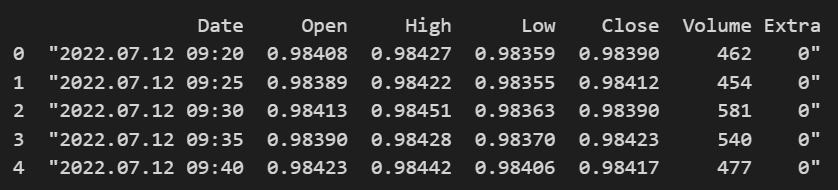
\includegraphics[scale=1.0]{gambar/positional encoding.png} 
\caption{Preprocessing \& Input Encoding}
\label{fig:positionalencoding}
\end{figure}

Gambar \ref{fig:positionalencoding} menunjukkan bagaimana positional encoding ditambahkan ke dalam data input. Positional encoding ini akan memberikan informasi tentang posisi setiap elemen dalam sekuens, sehingga model dapat memahami urutan data dengan lebih baik.

Adapun bentuknya akan disesuaikan dengan kebutuhan input yang akan digunakan dalam pengujian model yang akan dilakukan. Pada penelitian ini, penulis menggunakan 12, 24, dan 36 timestamp sebagai input untuk model Time Series Transformer.

\subsection{MinMax Scaler}
Pada dataset yang terdiri atas berbagai fitur dengan rentang nilai yang berbeda-beda, model machine learning dapat mengalami kesulitan dalam melakukan proses pelatihan. Fitur dengan rentang nilai yang lebih besar dapat mendominasi perhitungan jarak (\textit{distance}) atau bobot (\textit{weight}) dalam algoritma tertentu, sehingga menghasilkan bias pada hasil prediksi. Oleh karena itu, normalisasi diperlukan untuk menyeragamkan skala nilai seluruh fitur. Berikut merupakan formula yang digunakan untuk melakukan normalisasi data menggunakan MinMax Scaler:

\begin{equation}
  X_{Scaled} = \frac{X - X_{Min}}{X_{Max}-X_{Min}}
\end{equation}

Dimana : 
\begin{itemize}
    \item \( X_{Scaled} \) adalah nilai yang telah dinormalisasi.
    \item \( X \) adalah nilai asli dari fitur.
    \item \( X_{Min} \) adalah nilai minimum dari fitur tersebut.
    \item \( X_{Max} \) adalah nilai maksimum dari fitur tersebut.
\end{itemize}
Normalisasi ini akan mengubah nilai fitur menjadi rentang antara 0 dan 1, sehingga semua fitur memiliki skala yang seragam. Hal ini penting untuk memastikan bahwa model machine learning dapat belajar dari data dengan lebih efektif, tanpa terpengaruh oleh perbedaan skala antar fitur.

\subsection{Split Data}
Pada tahap ini, dataset dibagi menjadi dua bagian, yaitu data latih (\textit{training set}) dan data uji (\textit{testing set}). Tujuan dari pembagian ini adalah untuk memastikan bahwa model machine learning yang dibangun dapat diuji performanya menggunakan data yang belum pernah dilihat sebelumnya, sehingga hasil evaluasi lebih objektif dan akurat.

\begin{figure} [H] \centering
  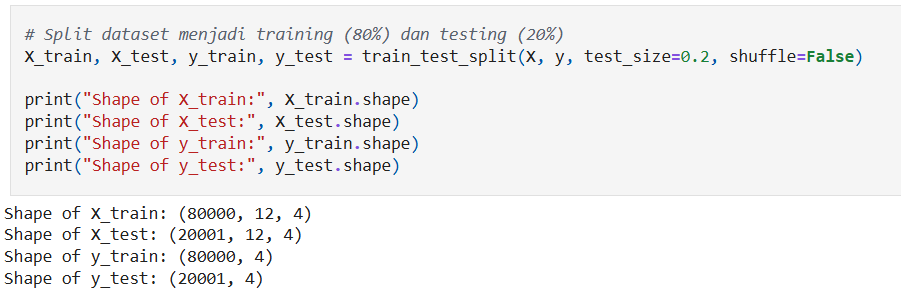
\includegraphics[scale=1.0]{gambar/splitdata.png} 
  \caption{Split Data}
  \label{fig:split_data}
\end{figure}

Dataset berjumlah 100.001,data uji sebanyak 20.001 dan data latih sebanyak 80.000. Parameter \textbf{shuffle=False} menentukan bahwa data tidak diacak sebelum dibagi yang berguna untuk menjaga urutan data dan tidak terjadi kebocoran data antara data latih dan data uji.

\section{Transformer Layer}
Pada tahap ini, data yang telah disiapkan sebelumnya akan diproses melalui dua komponen utama dari arsitektur Transformer, yaitu self-attention mechanism dan feed-forward network.

\subsection{Self-Attention Mechanism}
Self - attention adalah mekanisme dalam arsitektur Transformer yang memungkinkan untuk menilai pentingnya setiap elemen dalam sekuens input relatif terhadap elemen lainnya. Self-attention digunakan untuk menangkap dependensi temporal antara data pada waktu yang berbeda. Formula yang digunakan dalam metode ini sebagai berikut.

\begin{equation}
  Attention(Q,K,V) = Softmax(\frac{QK^{T}}{\sqrt{d_{k}}})V
\end{equation}
Self-Attention membutuhkan tiga matriks:
\begin{itemize}
  \item \textbf{Query(Q)}: Representasi elemen yang ingin mencari perhatian dari elemen lain.
  \item \textbf{Key(K)}: Representasi elemen-elemen yang memberikan sinyal penting atau tidaknya.
  \item \textbf{Value(V)}: Informasi yang akan dipertimbangkan atau diambil berdasarkan bobot perhatian.
\end{itemize}

Matriks \( Q \), \( K \), dan \( V \) dibentuk dengan mengalikan input \( X \) dengan matriks bobot \( W_Q \), \( W_K \), dan \( W_V \):

\begin{equation}
Q = XW_Q \quad K = XW_K \quad V = XW_V
\end{equation}

\subsubsection{Tahap-Tahap Perhitungan Self-Attention}
\begin{enumerate}
    \item \textbf{Menghitung Skor Kesamaan(Dot Product)}
    Untuk setiap elemen dalam sekuens, hitung kesamaan antara query dan key menggunakan dot product:
      \begin{equation}
        Score(Q,K) = Q \cdot K^{T}
      \end{equation}

    Ini menghasilkan matriks ukuran \( n \) \( x \) \ \( n \), dimana \( n \) adalah panjang sekuens.

    \item\textbf{Scaling(Normalisasi)}
    Skor yang dihasilkan dibagi dengan akar kuadrat dari dimensi key \(\sqrt{d_k} \)  untuk menjaga stabilitas numerik, terutama ketika nilai dot product besar:
    \begin{equation}
      Scaled Score = (\frac{QK^{T}}{\sqrt{d_{k}}})
    \end{equation}

    
    \item\textbf{(Softmax)}
    Gunakan fungsi softmax pada skor yang sudah diskalakan untuk mengubahnya menjadi probabilitas yang menunjukkan pentingnya setiap elemen dalam sekuens
    \begin{equation}
      Attention Weights = Softmax(\frac{QK^{T}}{\sqrt{d_{k}}})V
    \end{equation}
    Softmax memastikan bahwa semua bobot perhatian bernilai antara 0 dan 1 dan jumlah totalnya adalah 1.
    \item\textbf{Menghitung Weighted Sum (Agregasi Informasi)}
    Bobot perhatian tersebut kemudian digunakan untuk menghitung kombinasi linier dari matriks \textbf{Value (V):}
    \begin{equation}
      Attention Output = Attention Weights \cdot V
    \end{equation}
\end{enumerate}

\subsubsection{Multi-Head Self-Attention}
Pada layer ini, Time Series Transformer juga mengolah data menggunakan multi head dengan cara menggabungkan beberapa “head” (proses self-attention yang independen). Setiap head memungkinkan model untuk fokus pada berbagai bagian dari input sequence secara paralel, menangkap berbagai tipe hubungan atau pola dalam data.Berikut merupakan formula yang digunakan.
    \begin{equation}
      MultiHead(Q,K,V)=Concat(head_{1}, ...,head_{h})W_{O}
    \end{equation}
Setiap head melakukan self-attention secara independen, dan hasilnya digabungkan kembali dengan matriks bobot \( W_O \).

\subsection{Feed Forward Network}
Lapisan ini adalah bagian dari layer transformer. FFN bekerja secara independen di setiap posisi dalam sequence dan bertujuan untuk memperkuat kemampuan model dalam memproses representasi data yang diperoleh dari proses sebelumnya yaitu self-attention. Setelah self-attention menangkap hubungan antar elemen dalam sequence, FFN memperkuat dan memperkaya representasi tersebut.FFN bekerja pada setiap posisi dalam sequence secara paralel, tidak seperti self-attention yang mempertimbangkan konteks antar posisi.Dengan fungsi ini,FFN akan belajar hubungan non-linear dalam data time series, seperti pola musiman atau anomali.

FFN terdiri dari dua lapisan linear dengan fungsi aktivasi non-linear di antaranya. Formula yang digunakan dalam feed forward network adalah sebagai berikut:
\begin{equation}
  FFN(x) = \sigma(xW_1 + b_1)W_2 + b_2
\end{equation}
Di mana:
\begin{itemize}
    \item \( x \) adalah input dari layer self-attention.
    \item \( W_1 \) dan \( W_2 \) adalah matriks bobot untuk lapisan pertama dan kedua.
    \item \( b_1 \) dan \( b_2 \) adalah bias untuk lapisan pertama dan kedua.
    \item \( \sigma \) adalah fungsi aktivasi non-linear, seperti ReLU atau GELU.
\end{itemize}
Feed Forward Network ini akan mengubah representasi yang dihasilkan oleh self-attention menjadi representasi yang lebih kaya dan kompleks, sehingga model dapat menangkap pola-pola yang lebih dalam dalam data time series. Proses ini dilakukan secara paralel untuk setiap posisi dalam sequence, sehingga efisien dalam hal komputasi.

\subsection{Residual \& Normalization}
Residual Connection dan Layer Normalization adalah dua komponen penting yang membantu stabilitas pelatihan dan mempercepat konvergensi model. Kedua komponen ini bekerja untuk memastikan bahwa representasi data tidak hilang atau terdistorsi selama proses transformasi melalui berbagai layer.

\newpage
\subsubsection*{3.4.3.1 Residual Connection}
Residual connection adalah teknik yang memungkinkan input awal suatu layer untuk langsung ditambahkan ke output layer tersebut, sebelum diteruskan ke proses berikutnya.Memungkinkan gradien untuk mengalir dengan lebih baik ke layer sebelumnya selama backpropagation, sehingga membantu pelatihan model yang lebih dalam.Model belajar lebih cepat karena input mentah tetap tersedia di setiap layer.Memastikan bahwa informasi penting dari input asli tidak hilang selama proses transformasi.Formula dari residual connection adalah: 

\begin{equation}
Output = f(x) + x
\end{equation}

Di mana: 
\begin{itemize}
        \item \( x \) adalah input layer.
        \item \( f \)(\( x \)) adalah hasil dari operasi di layer self-attention dan feed-forward network.
    \end{itemize}

% \begin{align}
% Output &= LayerNorm(x) + Self-Attention(x) \\
% Output &= LayerNorm(x) + Feed-Forward(x)
% \end{align}

\subsubsection*{3.4.3.2 Normalization}
Normalization adalah teknik yang digunakan untuk meningkatkan kestabilan dan mempercepat konvergensi dalam pelatihan jaringan saraf, terutama untuk model yang lebih dalam dan kompleks seperti Transformer.Normalization diterapkan untuk menormalkan output dari setiap lapisan sehingga distribusi data tetap stabil selama proses pelatihan. Hal ini sangat penting dalam menangani fluktuasi data time series, seperti harga pasar modal yang seringkali sangat volatil. Data Time Series seringkali memiliki fluktuasi yang tajam. Dengan normalisasi, distribusi data menjadi lebih stabil, memudahkan model dalam menangani variasi yang tinggi dalam data.Normalisasi juga membantu mengurangi ketergantungan pada cara parameter jaringan diinisialisasi, yang sering kali menjadi tantangan dalam pelatihan model yang dalam.Model lebih cepat mencapai konvergensi karena tidak terpengaruh oleh perubahan besar dalam distribusi data antar batch. Normalization mempunyai formula sebagai berikut

\begin{equation}
    \hat{x} = \frac{x - \mu}{\sigma}
\end{equation}

Layer Normalization menghitung rata-rata (\( u \)) dan standar deviasi ($\sigma$) dari fitur di dalam suatu lapisan dan kemudian menormalisasi output dari lapisan tersebut

\newpage
\subsection{Visualisasi Arsitektur Model TST}
Untuk memberikan gambaran yang lebih jelas mengenai alur pemrosesan data pada model Transformer yang digunakan, berikut ditampilkan visualisasi arsitektur lengkap dari model Time Series Transformer (TST) yang telah dibangun. Visualisasi ini mencerminkan urutan layer dari input OHLC 12 timestep hingga output prediksi 5 timestep ke depan.

\begin{figure}[H]
    \centering
    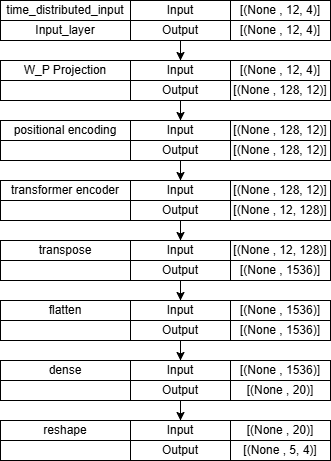
\includegraphics[scale=0.65]{gambar/tstars.png} 
    \caption{Arsitektur Model Time Series Transformer (TST)}
    \label{fig:tst_architecture}
\end{figure}

Dari gambar di atas dapat dilihat bahwa input berupa sekuens data OHLC dengan panjang 12 timestep terlebih dahulu diproyeksikan ke dimensi baru, diberi positional encoding, dan kemudian diproses oleh encoder transformer. Hasilnya kemudian dirapikan melalui operasi \textit{transpose}, \textit{flatten}, dan \textit{dense}, sebelum akhirnya dibentuk ulang menjadi output prediksi OHLC untuk 5 timestep ke depan.


\section{Model Pembanding}
Dalam tugas akhir ini model TST yang telah dibangun sebelumnya akan dibandingkan dengan model dengan arsitektur LSTM pada subbab ini. Adapun model pembanding ini disesuaikan jumlah timestampnya untuk dibandingkan dengan model TST yang memiliki Timestamp yang serupa. Adapun ketiga jenis arsitektur modelnya yaitu sebagai berikut.

\subsection{Arsitektur LSTM Model Pertama}
Pada gambar \ref{fig:lstm1} merupakan arsitektur LSTM yang akan digunakan untuk membangun model pembanding. Visualisasi ini bertujuan untuk menampilkan input dan output dari arsitektur yang telah ditetapkan penulis pada model pembanding ini. Adapun dataset yang digunakan telah melalui proses yang serupa dengan model TST sehingga dapat digunakan untuk menjadi pembanding dari model TST yang akan digunakan.

\begin{figure} [H] \centering
    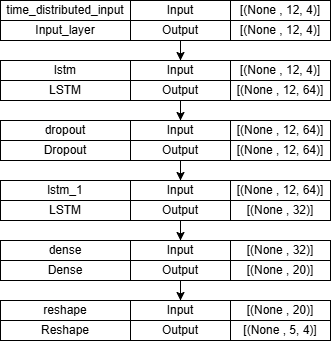
\includegraphics[scale=0.65]{gambar/lstmmodel1.png} 
    \caption{Arsitektur LSTM Model 1}
    \label{fig:lstm1}
\end{figure}

Adapun penjelasan dari setiap lapisan model adalah sebagai berikut:

\begin{itemize}
    \item \textbf{LSTM Layer 1:} Lapisan LSTM pertama terdiri dari 64 unit dan menerima input dengan dimensi (12, 4). Layer ini memproses seluruh sekuens input dan mengembalikan keluaran untuk setiap timestep, yang membantu model memahami hubungan jangka pendek dan menengah antar titik data.
    
    \item \textbf{Dropout:} Setelah LSTM pertama, diterapkan dropout sebesar 20\% untuk mencegah model mengalami overfitting, terutama saat proses pelatihan.
    
    \item \textbf{LSTM Layer 2:} Lapisan LSTM kedua terdiri dari 32 unit dan hanya mengembalikan output dari timestep terakhir. Di sini, model menyimpulkan informasi penting dari keseluruhan input sebelumnya dalam satu vektor.
    
    \item \textbf{Dense Layer:} Lapisan Dense mengubah vektor hasil dari LSTM kedua menjadi vektor dengan panjang 20, yang mewakili 5 timestep ke depan dengan masing-masing 4 fitur (5 × 4 = 20).
    
    \item \textbf{Reshape Layer:} Vektor output dari Dense kemudian diubah menjadi bentuk matriks (5, 4), sehingga model dapat menghasilkan prediksi OHLC untuk lima waktu berikutnya.
\end{itemize}

Arsitektur ini digunakan sebagai baseline atau model dasar untuk membandingkan performanya dengan model Transformer yang telah dibahas pada bab sebelumnya. Struktur yang sederhana namun efektif ini akan membantu dalam mengevaluasi sejauh mana keunggulan pendekatan Transformer dalam memprediksi data deret waktu.

\subsection{Arsitektur LSTM Model Kedua}
Model LSTM kedua memiliki arsitektur yang lebih kompleks dibandingkan model pertama. Arsitektur ini menggunakan tiga lapisan LSTM yang disusun secara berurutan (stacked LSTM), dengan tujuan untuk memperdalam pemahaman model terhadap pola dalam data historis. Semakin banyak lapisan yang digunakan, maka semakin dalam model dapat menangkap pola jangka pendek maupun jangka panjang dalam data deret waktu.

Visualisasi arsitektur model ditunjukkan pada Gambar \ref{fig:lstm2}. Sama seperti model sebelumnya, input yang digunakan adalah data OHLC selama 12 timestep dengan interval 5 menit. Model ini akan menghasilkan prediksi OHLC untuk 5 langkah waktu ke depan, atau setara dengan 25 menit prediksi.

\begin{figure} [H] \centering
    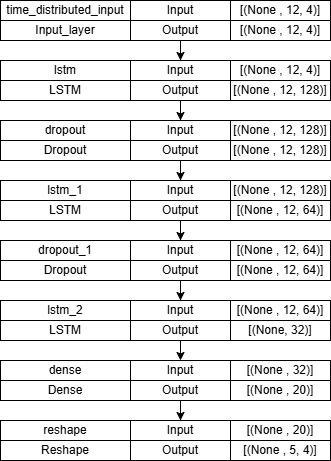
\includegraphics[scale=0.65]{gambar/lstmmodel2.png} 
    \caption{Arsitektur LSTM Model 2}
    \label{fig:lstm2}
\end{figure}

Berikut adalah penjelasan dari setiap lapisan model:

\begin{itemize}
    \item \textbf{LSTM Layer 1:} Lapisan pertama terdiri dari 128 unit LSTM. Layer ini menerima input berbentuk (12, 4), lalu mengembalikan output untuk setiap timestep (\textit{return\_sequences=True}) agar dapat diteruskan ke layer berikutnya.
    
    \item \textbf{Dropout:} Setelah LSTM pertama, digunakan dropout sebesar 30\% untuk mencegah overfitting.
    
    \item \textbf{LSTM Layer 2:} Lapisan kedua memiliki 64 unit LSTM dan juga mengembalikan urutan output (\textit{return\_sequences=True}). Penambahan layer ini membantu model menangkap pola yang lebih dalam dalam data.
    
    \item \textbf{Dropout:} Dropout kembali diterapkan dengan rasio 30\% sebagai upaya regularisasi.
    
    \item \textbf{LSTM Layer 3:} Lapisan terakhir terdiri dari 32 unit dan hanya mengembalikan hasil dari timestep terakhir (\textit{return\_sequences=False}). Layer ini menyaring dan merangkum semua informasi yang diperoleh dari dua lapisan sebelumnya.
    
    \item \textbf{Dense Layer:} Lapisan Dense mengubah hasil dari LSTM ketiga menjadi vektor berdimensi 20, yang merepresentasikan 5 timestep ke depan dengan masing-masing 4 fitur.
    
    \item \textbf{Reshape Layer:} Vektor output kemudian diubah menjadi matriks berukuran (5, 4), sesuai dengan struktur output prediksi OHLC.
\end{itemize}

Model kedua ini dirancang untuk menguji apakah penggunaan arsitektur LSTM bertingkat (stacked) dapat meningkatkan akurasi prediksi dibandingkan dengan model LSTM tunggal yang lebih sederhana. Kedalaman model memungkinkan pembelajaran representasi yang lebih kompleks, namun juga berisiko overfitting jika tidak diatur dengan baik.

\subsection{Arsitektur LSTM Model 3}
Model LSTM ketiga menggunakan pendekatan \textit{Bidirectional LSTM}, yaitu variasi dari LSTM yang mampu memproses data urutan dalam dua arah, yakni maju dan mundur. Pendekatan ini memungkinkan model memahami konteks secara lebih luas dari urutan data yang diberikan, sehingga diharapkan dapat meningkatkan kualitas prediksi.

Model ini tetap menggunakan 12 timestep sebagai input, masing-masing berisi 4 fitur (OHLC), dan menghasilkan prediksi untuk 5 timestep ke depan. Visualisasi dari arsitektur model ditunjukkan pada Gambar \ref{fig:lstm3}.

\begin{figure} [H] \centering
    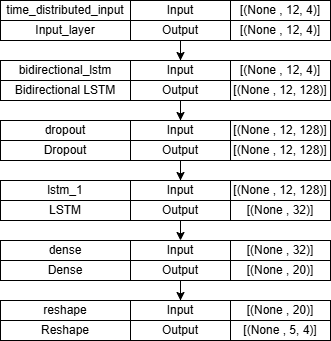
\includegraphics[scale=0.65]{gambar/lstmmodel3.png} 
    \caption{Arsitektur LSTM Model 3 (Bidirectional)}
    \label{fig:lstm3}
\end{figure}

Berikut adalah penjelasan dari setiap lapisan dalam model ini:

\begin{itemize}
    \item \textbf{Bidirectional LSTM:} Lapisan pertama adalah LSTM dengan 64 unit yang dibungkus oleh layer \textit{Bidirectional}. Artinya, model akan memproses data dari awal ke akhir (forward) dan dari akhir ke awal (backward) secara bersamaan. Output dari kedua arah akan digabung dan diteruskan ke layer berikutnya. Output dari layer ini memiliki bentuk sekuensial karena \textit{return\_sequences=True}.
    
    \item \textbf{Dropout:} Dropout sebesar 30\% digunakan setelah Bidirectional LSTM untuk mengurangi risiko overfitting.
    
    \item \textbf{LSTM Layer:} Lapisan LSTM biasa dengan 32 unit yang hanya mengembalikan hasil pada timestep terakhir. Layer ini bertugas merangkum informasi dari output sekuensial sebelumnya menjadi satu vektor representasi.
    
    \item \textbf{Dense Layer:} Layer Dense akan mengubah vektor hasil dari LSTM menjadi 20 unit output, mewakili 5 timestep dengan masing-masing 4 fitur.
    
    \item \textbf{Reshape Layer:} Output kemudian diubah menjadi bentuk (5, 4), sesuai dengan struktur prediksi OHLC yang diinginkan.
\end{itemize}

Model ini dirancang untuk menguji sejauh mana pendekatan dua arah (bidirectional) dapat memberikan hasil yang lebih baik dibandingkan LSTM biasa atau stacked LSTM. Dengan mempertimbangkan konteks dari dua arah, diharapkan model lebih peka terhadap pola-pola harga yang kompleks pada data deret waktu.


% \begin{figure} [H] \centering
%     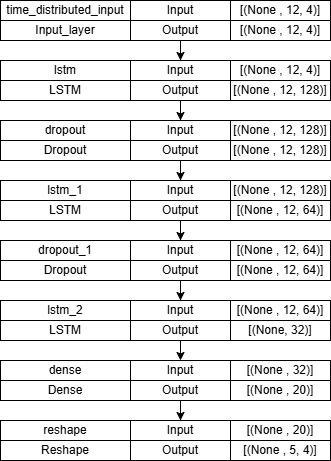
\includegraphics[scale=0.8]{gambar/lstmmodel2.png} 
%     \caption{Struktur Model LSTM Timestep 12 (Stacked LSTM)}
%     \label{fig:lstm2}
% \end{figure}
% \subsection{Arsitektur LSTM Timestep 12}
% Dapat dilihat dari gambar berikut ini merupakan arsitektur LSTM yang akan digunakan untuk membangun model pembanding. Visualisasi ini bertujuan untuk menampilkan input dan output dari arsitektur yang telah ditetapkan penulis pada model pembanding ini. Adapun dataset yang digunakan telah melalui proses yang serupa dengan model TST sehingga dapat digunakan untuk menjadi pembanding dari model TST yang akan digunakan. 
% % \begin{figure} [H] \centering
% %   % Nama dari file gambar yang diinputkan
% %     \includegraphics[scale=0.8]{gambar/summarylstm12.png} 
% %     \caption{Struktur Model LSTM Timestep 12}
% %     \label{fig:label_gambar}
% % \end{figure}

% % \begin{figure} [H] \centering
% %   % Nama dari file gambar yang diinputkan
% %     \includegraphics[scale=0.8]{gambar/lstm(12).jpeg} 
% %     \caption{Arsitektur Model LSTM Timestep 12}
% %     \label{fig:label_gambar}
% % \end{figure}

% Input model berasal dari data historis OHLC (Open, High, Low, Close) yang dikumpulkan setiap 5 menit. Model akan melihat ke belakang selama 1 jam (12 data berturut-turut × 5 menit), sehingga total input berisi 12 timestamp yang masing-masing memuat 4 fitur Harga yaitu Open, High, Low, dan Close.

% Setelah data dinormalisasi agar berada dalam rentang yang seragam, data tersebut diproses oleh LSTM pertama dengan 64 unit. LSTM ini akan mengubah 4 fitur harga per waktu menjadi representasi fitur berdimensi 64, sambil tetap mempertahankan urutan waktunya (karena return\_sequences=True). Selanjutnya, lapisan dropout diterapkan untuk mencegah overfitting dengan cara mengabaikan sebagian neuron saat pelatihan.

% Kemudian, hasil tersebut masuk ke LSTM kedua yang hanya mengambil output pada waktu terakhir (return\_sequences=False), sehingga menghasilkan sebuah vektor dengan 32 unit yang merangkum informasi pergerakan harga selama 1 jam terakhir. Lapisan dropout kembali digunakan untuk menjaga generalisasi model. Output dari LSTM kemudian diproses oleh lapisan Dense (fully connected) berukuran 32 unit, diikuti dengan lapisan output Dense berisi 4 unit yang merepresentasikan prediksi harga Open, High, Low, dan Close berikutnya.

% \subsection{Arsitektur LSTM Timestep 24}
% % \begin{figure} [H] \centering
% %   % Nama dari file gambar yang diinputkan
% %     \includegraphics[scale=0.8]{konten/summarylstm24.png} 
% %     \caption{Struktur Model LSTM Timestep 24}
% %     \label{fig:label_gambar}
% % \end{figure}
% % \begin{figure} [H] \centering
% %   % Nama dari file gambar yang diinputkan
% %     \includegraphics[scale=0.8]{konten/lstm24.jpeg} 
% %     \caption{Arsitektur Model LSTM Timestep 24}
% %     \label{fig:label_gambar}
% % \end{figure}
% Pada arsitektur ini masih sama dengan arsitektur sebelumnya tetapi dengan input timestep 24, yaitu data akan mem-proses data per 2 jam ( 24 data x 5 menit), total input berisi 24 timestep yang masing masing memuat 4 fitur harga yaitu, Open,High,Low,Close.
% Setelah data dinormalisasi,akan diproses dengan mengubah menjadi fitur berdimensi 64 dan masih mempertahankan urutan waktunya,dan  dilanjutkan ke lapisan dropout untuk mencehag overfitting. Kemudian dilanjutkan ke LSTM kedua yang mengambil output waktu terakhir,sehingga menghasilkan vektor 32 unit berdasarkan pergerakan harga 1 jam terakhir, dilanjutkan dengan lapisan dropout. Output dari LSTM diproses lapisan Dense berukuran 32 units, yang berisi prediksi harga Open,High,Low,Close.

% \subsection{Arsitetur LSTM Timestep 36}

% % \begin{figure} [H] \centering
% %   % Nama dari file gambar yang diinputkan
% %     \includegraphics[scale=0.8]{konten/summarylstm36.png} 
% %     \caption{Struktur Model LSTM Timestep 36}
% %     \label{fig:label_gambar}
% % \end{figure}
% % \begin{figure} [H] \centering
% %   % Nama dari file gambar yang diinputkan
% %     \includegraphics[scale=0.8]{konten/lstm36.jpeg} 
% %     \caption{Arsitektur Model LSTM Timestep 36}
% %     \label{fig:label_gambar}
% % \end{figure}

% Arsitektur ini sama dengan arsitektur sebelumnya, perubahan yang ada hanya di bagian timestep, timestep yang digunakan pada arsitektur ini adalah 36(5 menit x 36), model akan memproses data per 3 jam dengan fitur Harga Open, High, Low, Close , dan membandingkan hasil prediksi dengan timestep 12, dan 24.


% Secara keseluruhan, arsitektur ini mengandalkan memori jangka panjang dan pendek dari LSTM untuk memahami pola pergerakan harga dalam waktu singkat, dan memberikan prediksi yang mencakup keempat komponen harga utama pada candle berikutnya.


\subsection{Inverse Scale}
Setelah model machine learning melakukan proses prediksi terhadap data uji, nilai hasil prediksi yang dihasilkan masih dalam skala hasil normalisasi (dalam hal ini menggunakan MinMaxScaler dengan rentang 0 hingga 1). Oleh karena itu, nilai tersebut perlu dikembalikan ke skala aslinya agar dapat dibandingkan secara langsung dengan data harga sebenarnya.

\begin{figure} [H] \centering
  % Nama dari file gambar yang diinputkan
    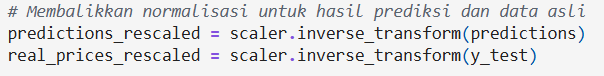
\includegraphics[scale=1.0]{gambar/inverse scaler.png} 
    \caption{Inverse Scaler}
    \label{fig:InverseScaler}
\end{figure}


\subsection{Output}
Output layer berfungsi untuk menghasilkan prediksi berdasarkan hasil yang diperoleh dari model setelah proses transformasi dilakukan. Output layer biasanya memiliki satu unit untuk setiap langkah waktu prediksi yang dihasilkan.Memprediksi harga untuk beberapa langkah ke depan, jumlah neuron di output layer akan sesuai dengan jumlah langkah yang diprediksi. Output layer sering kali menggunakan fungsi aktivasi linear (ReLU, atau tanpa fungsi aktivasi). Ini memungkinkan model untuk menghasilkan nilai kontinu yang sesuai dengan harga pasar modal. Dimensi output layer dapat disesuaikan dengan kebutuhan prediksi. Dalam kasus harga pasar modal, output layer akan mengeluarkan nilai yang menunjukkan harga pasar modal pada waktu tertentu.Dimensi output ini akan berupa Candle stick dengan panjang yang sesuai dengan jumlah langkah waktu yang akan diprediksi. Candle stick ini akan merepresentasikan harga Open, High, Low, dan Close untuk setiap langkah waktu yang diprediksi. Candle stick ini dibuat menggunakan \textit{mplfinance} yang merupakan library untuk visualisasi data pasar modal.

\subsubsection*{3.5.5.1 Grafik Output}
Setelah data melewati encoder dan decoder dan di normalisasi, output layer akan memberikan hasil prediksi berdasarkan informasi yang telah dipelajari oleh model.Untuk prediksi harga pasar modal, model akan menghasilkan harga yang diprediksi untuk langkah waktu tertentu ke depan berdasarkan pola yang telah dipelajari dari data historis.

\begin{figure} [H] \centering
  % Nama dari file gambar yang diinputkan
    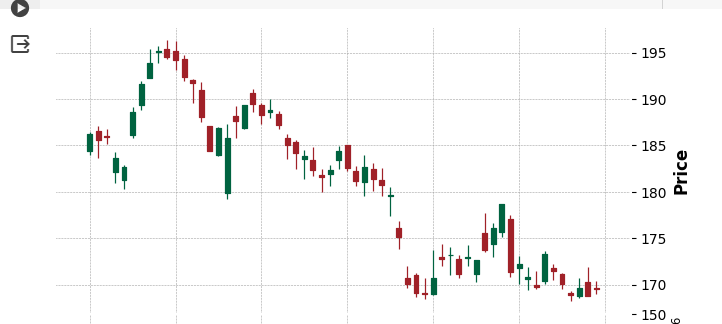
\includegraphics[scale=0.6]{gambar/outputlay.png} 
    \caption{Output Layer}
    \label{fig:outputgraf}
\end{figure}

Gambar \ref{fig:outputgraf} merupakan output layer yang akan ditampilkan dari hasil prediksi. Setiap waktunya akan di tampilkan dengan sebuah candle stick.

\subsection{Loss Function}
Untuk mengevaluasi model yang telah dilatih time series transformer,akan digunakan Mean Squares Error(MSE). Dari hasil yang akan dikeluarkan MSE dapat terlihat hasil performa model Time Series Transformer dalam memprediksi harga pasar modal.

\subsubsection*{3.5.6.1 Mean Squared Error (MSE)}
Mean Squared Error (MSE) adalah fungsi loss yang umum digunakan dalam masalah regresi, termasuk untuk model seperti Time Series Transformer yang memprediksi harga pasar modal. MSE mengukur seberapa besar perbedaan antara nilai yang diprediksi oleh model dan nilai aktual yang diamati. Semakin kecil nilai MSE, semakin baik model dalam memprediksi harga. MSE mempunyai formula sebagai berikut

\[
A = \sum_{i=1}^{n} \left( \frac{1}{2} x_i^2 + \sqrt{x_i + 1} \right)
\]

\begin{itemize}
    \item \( y_{pred}(i) \) adalah prediksi harga pasar modal pada data ke-i.
    \item \( y_{true}(i) \) adalah harga pasar modal yang sebenarnya pada data ke-i.
    \item \( n \) adalah jumlah data dalam batch.
\end{itemize}

Dalam prediksi harga pasar modal, harga pasar modal akan bernilai kontinu. MSE cocok digunakan karena menghitung rata-rata kuadrat selisih antara prediksi dan nilai aktual. MSE memberikan penalti yang lebih besar untuk prediksi yang jauh dari nilai sebenarnya, sehingga model cenderung lebih berhati-hati dalam menghasilkan prediksi yang jauh dari harga sebenarnya.



\cleardoublepage

% Bab 4 pengujian dan analisis
\chapter{PENGUJIAN DAN ANALISIS}
\label{chap:pengujiananalisis}

% Ubah bagian-bagian berikut dengan isi dari pengujian dan analisis

Pada penelitian ini dipaparkan \lipsum[1][1-5]

\section{Skenario Pengujian}
\label{sec:skenariopengujian}

Pengujian dilakukan dengan \lipsum[1-2]

\section{Evaluasi Pengujian}
\label{sec:analisispengujian}

Dari pengujian yang \lipsum[1]

% Contoh pembuatan tabel
\begin{longtable}{|c|c|c|}
  \caption{Hasil Pengukuran Energi dan Kecepatan}
  \label{tb:EnergiKecepatan}                                   \\
  \hline
  \rowcolor[HTML]{C0C0C0}
  \textbf{Energi} & \textbf{Jarak Tempuh} & \textbf{Kecepatan} \\
  \hline
  10 J            & 1000 M                & 200 M/s            \\
  20 J            & 2000 M                & 400 M/s            \\
  30 J            & 4000 M                & 800 M/s            \\
  40 J            & 8000 M                & 1600 M/s           \\
  \hline
\end{longtable}

\lipsum[2-4]

\cleardoublepage

% Bab 5 penutup
\chapter{PENUTUP}
\label{chap:penutup}

% Ubah bagian-bagian berikut dengan isi dari penutup

\section{Kesimpulan}
\label{sec:kesimpulan}

Berdasarkan hasil pengujian yang \lipsum[1][1-3] sebagai berikut:

\begin{enumerate}[nolistsep]

  \item Pembuatan \lipsum[2][1-3]

  \item \lipsum[2][4-6]

  \item \lipsum[2][7-10]

\end{enumerate}

\section{Saran}
\label{chap:saran}

Untuk pengembangan lebih lanjut pada \lipsum[1][1-3] antara lain:

\begin{enumerate}[nolistsep]

  \item Memperbaiki \lipsum[2][1-3]

  \item \lipsum[2][4-6]

  \item \lipsum[2][7-10]

\end{enumerate}

\cleardoublepage

\chapter*{DAFTAR PUSTAKA}
\addcontentsline{toc}{chapter}{DAFTAR PUSTAKA}
\renewcommand\refname{}
\vspace{2ex}
\renewcommand{\bibname}{}
\begingroup
    \def\chapter*#1{}
    \printbibliography
\endgroup
\cleardoublepage

% Biografi penulis
\begin{center}
  \Large
  \textbf{BIOGRAFI PENULIS}
\end{center}

\addcontentsline{toc}{chapter}{BIOGRAFI PENULIS}

\vspace{2ex}

\begin{wrapfigure}{L}{0.3\textwidth}
  \centering
  \vspace{-3ex}
  % Ubah file gambar berikut dengan file foto dari mahasiswa
  
\includegraphics[width=0.3\textwidth]{gambar/elon.jpg}
  \vspace{-4ex}
\end{wrapfigure}

% Ubah kalimat berikut dengan biografi dari mahasiswa
\name{}, lahir pada \lipsum[1]

\lipsum[2]

\cleardoublepage

\end{document}
